% Chapter 5

\begin{savequote}[\quotewidth] There are no significant technical limitations to column
temperature programming in the order of a few hundred degrees per minute and
equally rapid cool-down rates.
\qauthor{Wolfgang Bertsch, 1997}
\end{savequote}

\chapter[Instrumentation: Fast GC]{Instrumentation: Fast temperature programmed gas chromatography} % Main chapter title

\label{Chapter5} % For referencing this chapter elsewhere, use \ref{Chapter5}

The topic of this thesis is the development of a comprehensively coupled
(supercritical fluid × gas) chromatograph and its application to the analysis of
biodiesel. The discussion on the experimental work divides naturally into two
parts: the topic of the previous chapter is supercritical fluid chromatography
(SFC) and of this chapter it is gas chromatography (GC).

\section{Speed of analysis}
\label{sec:SpeedOfAnalysis}

The coupling between two chromatographs can be called \keyword{comprehensive} if
it meets the following criteria (as discussed in Section \ref{sec:SFCxGC}):
\begin{enumerate}
  \item Every part of the sample is separated by two distinct chromatographic processes.
  \item Equal percentages of all sample fractions are separated by the second process.	 
  \item Compounds resolved by the first dimension separation remain resolved.  
\end{enumerate} 

In principle, such a coupling could be implemented by manually or mechanically
collecting equal-sized fractions from a first \oneD chromatograph, and then
injecting a portion of each fraction into a different (\twoD) chromatograph. In
practice, such an approach would be slow, labour-intensive, expensive, and
error-prone. But reliable devices that can repeatedly collect and re-inject
fractions of eluate were invented. These devices became known as
\keyword{modulators} and made comprehensively coupled chromatography practical.
In continuous flow coupling, such as that found in GC×GC, the fraction
collection and \twoD injection happens during the uninterrupted \oneD
separation. In stopped-flow coupling as used in the SFC×GC chromatography
described here, the \oneD SFC separation is stopped after a fraction has been
collected. This fraction is separated on the \twoD GC column. After the \twoD
run is complete the SFC run is restarted and the next fraction is collected.

Fractions of the \oneD separation are collected at a rate which is determined
by the peak width on the \oneD chromatogram. To get adequate peak detection in
the \oneD chromatogram, at least \num{3} fractions of each \oneD peak should be
collected \autocite{Murphy1998}, but more would be better. For example, if the peaks
are \SI{3}{s} wide the collection rate should not be less than \SI{1}{\hertz}.
The rate of fractions collection is known as the \keyword{modulation rate} and
its inverse is the \keyword{modulation period} (\(P_M\)). In continuous-flow
coupling (\textit{e.g.} as found in GC×GC), the \twoD separation should be
completed in a time less than the modulation period. Evidently, this means that
the \twoD separation should be faster than the \oneD separation.

In stopped-flow coupling, the duration of the \twoD separation is largely
decoupled from the peak width of the of \oneD separation and, by implication,
the \oneD modulation period. In terms of the third criterion of comprehensive
coupling listed at the start of this section, as long as the resolution obtained
in the \oneD separation is not lost during the stopped-flow period, the duration
of the \twoD separation can be as long as it needs to be. In SFC the
longitudinal diffusion is low, so that in principle the \twoD GC runs in SFC×GC
need not be remarkably fast. In practice, however, \keyword{sample throughput}
of a chromatographic method needs to be acceptable. One of the major
determinants of sample throughput is \keyword{run time}, the time it takes from
when the sample is injected until the final compound has eluted. The judgement
of what is acceptable depends strongly on context: for finding the proverbial
biomarker for Alzheimer's disease very long run times might be acceptable, but
for routine analysis of a commodity biodiesel acceptable run times would
probably be short.
Therefore, when developing a practical SFC×GC chromatograph the aim should be to
make run times as short as possible.

The time it takes for a stopped-flow SFC×GC run can be calculated from

\[t_{T} = t_{^{1}D} ( 1 + \frac{t_{stopped}}{P_{M}} ) \]

where \(t_T\) is the total time, \(t_{^{1}D}\) is the run time the unmodulated
\oneD run would take, \(P_M\) is the \keyword{modulation period}, and
\(t_{stopped}\) is the duration of the SFC stopped-flow state, during which the
\twoD run is completed. With continuous-flow coupling (as in GC×GC) \(
t_{stopped}=0 \), so that \(t_{T} = t_{^{1}D}\).

Examining the expression shows that we can decrease \(t_T\) by increasing
\(P_M\), but there is limit to this: as the modulation period becomes longer the
separation obtained in the \oneD separation is decreased when fractions start
including first portions of two adjacent peaks and then more than one peak. So,
the only way to decrease the total run time is to reduce \(t_{stopped}\), the
GC run time. For example, if a typical SFC run takes \SI{20}{\minute} and fractions are
collected for every \SI{5}{\second} of SFC run, it means there will be \( 20
\times 60 / 5 = 240 \) fractions collected. Each of these fractions must be
injected into a GC chromatograph. If each GC run took \SI{1}{\minute}, the
SFC×GC run would last \SI{240}{\minute} = \SI{4}{\hour}. This is a very long run
time, and in the context of commodity biodiesel analysis the sample throughput
of such a chromatograph would probably be judged unacceptable.

Reducing the run time of the \twoD GC chromatography in SFC×GC means applying
the concepts of \keyword{fast chromatography}. Fast chromatography is the
discipline that studies the theories, experiments, and technologies that shorten
chromatographic run times.

\section{Fast gas chromatography theory}

Improving the speed of chromatographic separations is an aspect of
\keyword{optimization}. Optimization can be defined as ``the action of making
the best or most effective use of a situation or resource'' \autocite{OUP2019}.
``Making the most effective use" means that optimization has a
\keyword{goal}, which can be characterized by a numerical \keyword{criterion}
while subject to some \keyword{constraints}. The relative and variable amount
of ``resources'' used are \keyword{optimizing parameters}.

There are two kinds of optimization in chromatography: selectivity and kinetics.
The difference between them is not the goal of the optimization, but how the
optimizing parameters are selected. \keyword{Selectivity optimization} is the
process of selecting the best combination of stationary phase and analyte. The
optimization parameters are the different stationary phases and derivitization
methods available. \keyword{Kinetics optimization} is the process of selecting
the best combination of carrier gas, temperature, flow rate, column length,
column diameter, and stationary phase thickness. This differentiation between
selectivity optimization and kinetics optimization is not made on theoretical
grounds, but for practical reasons: selectivity optimization often involves the
discrete and expensive parameter of selecting a column, whereas the parameters
involved in kinetics optimization can often be adjusted continuously and
inexpensively. Selectivity optimization is guided by chemical thermodynamic
knowledge; kinetics optimization is guided by \keyword{chromatographic rate
theory}.

\begin{figure}
\centering
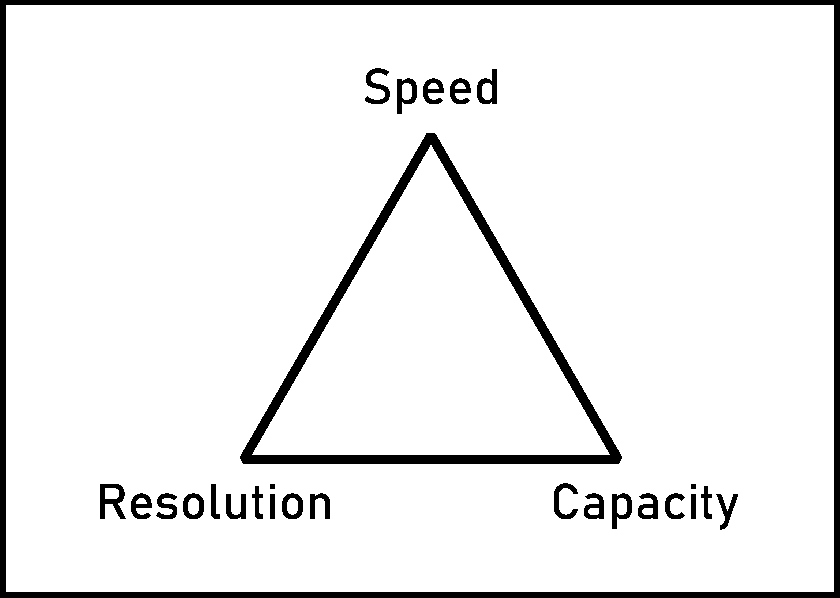
\includegraphics[width=0.75\textwidth]{Figures/Triangle.pdf}
\decoRule
\caption[Schematic diagram of a the chromatographer's trilemma.]{The chromatographer's trilemma.}
\label{fig:trilemma}
\end{figure}


Every chromatographer involved in a kinetics optimization has met the
chromatographer's trilemma (See Figure \ref{fig:trilemma}): Any chromatographic
method that involves decisions about speed, resolution, and capacity can
optimize only one at a time\footnote{This trilemma applies only to capillary
chromatography. When using packed columns, the capacity can be readily increased
by using a column with a larger diameter and a larger amount of packing.}. The
fastest chromatography will have low capacity and low resolution, the
chromatography giving the highest resolution will be slow with low capacity, and
the chromatography of a sample with a large amount of analyte will be slow
and have low resolution \autocite{Klee2002}. One way the chromatographer can
ease the grip of the trilemma is to decide what factor is least important for
the current problem, pick a value that is likely to satisfy most
conditions, keep it fixed, and then find an acceptable compromise between the
other two. In the development of the SFC×GC we decided to work with a fixed
sample capacity: we chose a capillary column with a \SI{0.25}{\milli\metre}
internal diameter and a \SI{0.25}{\micro\metre} stationary phase. With the
sample capacity held constant, it is now possible to optimize the system so that
it gives adequate resolution in the shortest possible time.

The \keyword{efficiency} of a column is given by the relationship \(E =
\frac{t_R}{\sigma} \), where \(t_R\) is the \keyword{retention time} of a peak,
and \(\sigma\) is its standard deviation, related to the \keyword{peak width}
\autocite{Blumberg2018}. The efficiency is a measure of how much the peak spread
during its transport through the column relative to distance it travelled, using
time as a proxy for distance. Efficiency is related to the more traditional but
less intuitive \keyword{number of plates} \(N\) through the expression \(N =
E^2\). The length of the column (\(L\)), divided by the square of the efficiency
gives the \keyword{plate height} (\(H\)). Plate height is a measure of how much
each unit of length of the column contributes to the separation: a lower \(H\)
means that the separation is more effective. The value of \(H\) in chromatographic
theory is that equations can be developed that express \(H\) as functions of the
adjustable parameters of kinetics optimization. Such functions help predict
suitable chromatographic conditions and set limits to the expected performance
of the separation.

Any chromatographic optimization goal must contain resolution as part of the
criteria. After all, the purpose of the activity is the separation of chemical
compounds. Traditionally, the first optimization taught is the optimization of
\(H\) as criterion, with the rate at which the carrier gas passes through the
column as the variable parameter. The rate can be characterized by either the
average gas velocity (\(\overline{u}\)) or the gas volume flow rate (\(F\)).
Traditionally \(\overline{u}\) has been used, because it can be conveniently
calculated from simple measurements: \(\overline{u} = L/t_m\), where \(t_m\) is
the \keyword{void time}, which is easily determined by measuring the retention
time of an unretained compound. In modern gas chromatographs \(F\) can be
continuously controlled by electronic pneumatic control (EPC) systems, and has
become a more convenient parameter.

Blumberg has developed the theory of optimized flow rate
\autocite{Blumberg1999}. He found that the function that describes plate height
in terms of flow rate can be simplified to two cases: a high-pressure drop and a
low-pressure drop. (A high pressure drop is defined as the case when the
difference in pressure between the inlet and outlet is much greater than the
outlet pressure, \(\Delta{p} \gg p_o\)). When the pressure drop is low

\(H = \frac{\displaystyle b}{\displaystyle F}+(c_1+c_2)F \)

and when the pressure drop is high

\(H = \frac{\displaystyle 9}{\displaystyle 8} \left(\frac{b}{F}+c_{1}F \right)+C_{2}\sqrt{F}\)

where \(c_1\), \(c_1\) and \(C_2\) are constants independent of \(F\).

When the layer of stationary phase is thin, also known as the \keyword{thin-film
case}, then \(c_2 = 0\) and \(C_2 = 0\), and

\(H = \frac{\displaystyle b}{\displaystyle F} + c_{1} F \) 

for the low pressure drop case and 

\(H = \frac{\displaystyle 9}{\displaystyle 8} \left(\frac{b}{F}+c_{1}F \right)\)

for the high pressure drop case. The low pressure drop case will be immediately
recognized as the \keyword{van Deemter equation}, and the high-pressure drop
case differs from it only by a factor of \num{1.125} (See Figure
\ref{fig:VanDeemter}).

\begin{figure}
\centering
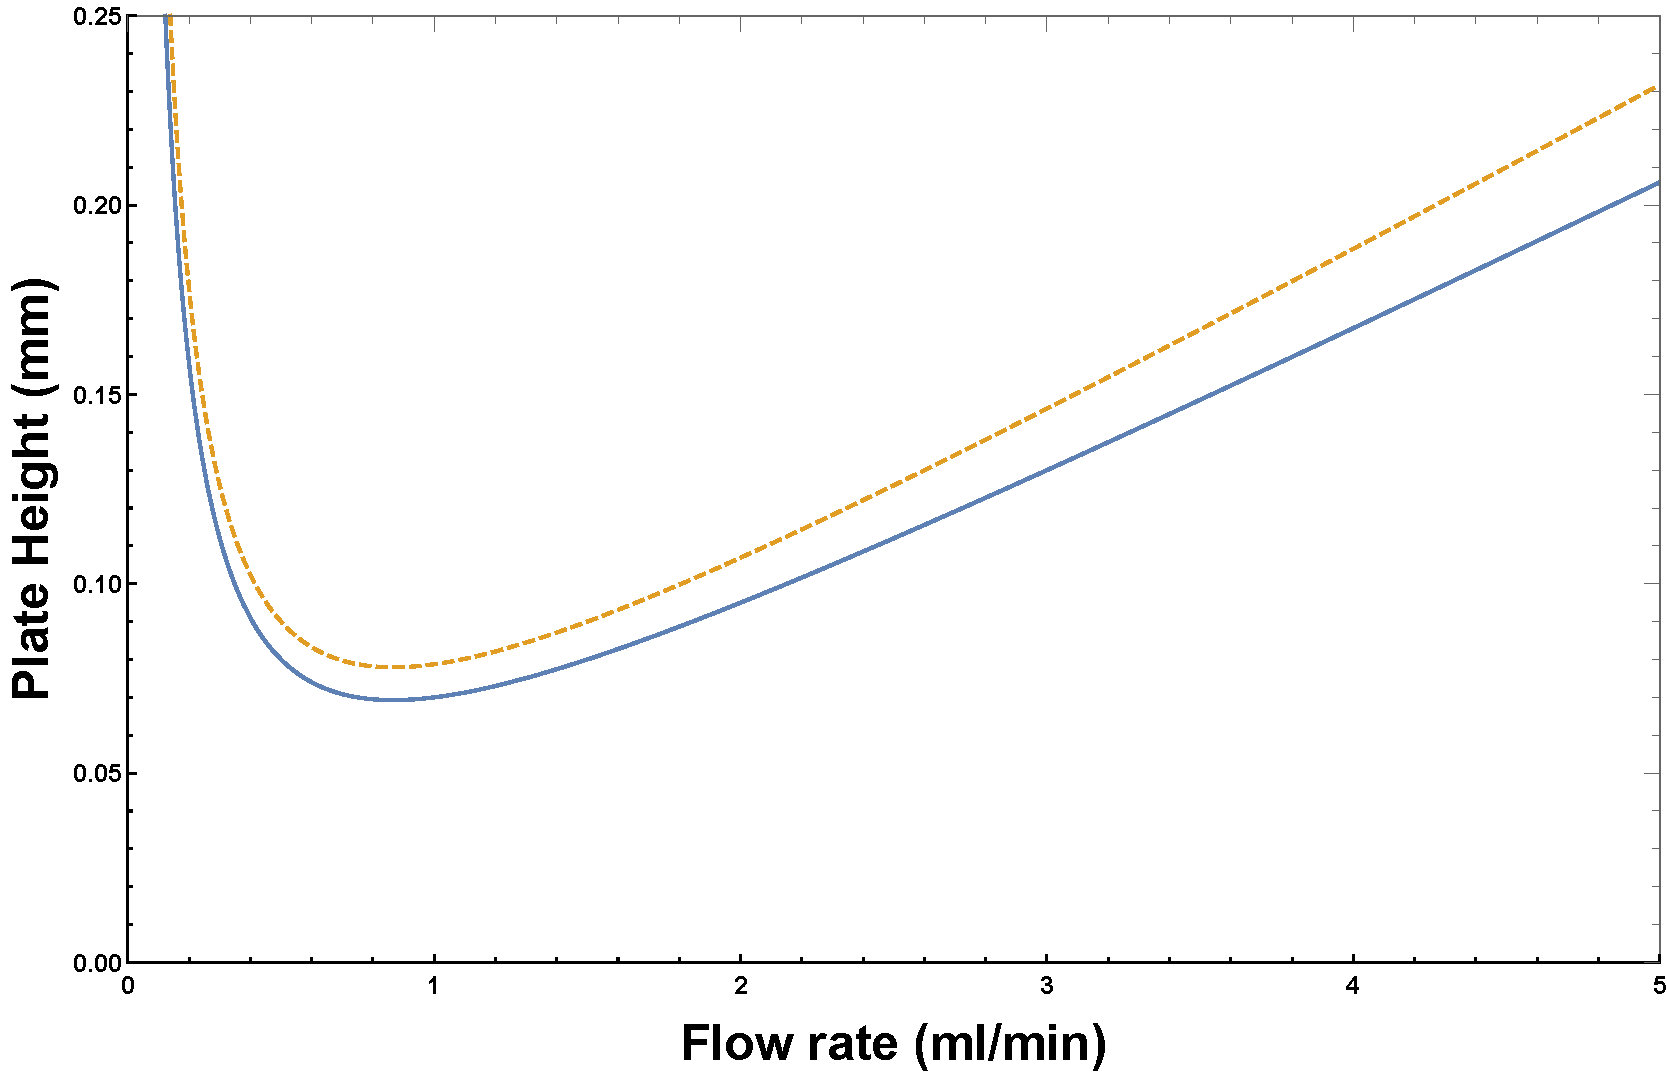
\includegraphics[width=0.75\textwidth]{Figures/VanDeemter.pdf}
\decoRule

\caption[A plot of H \textit{vs.} F]{A plot of H \textit{vs.} F. The solid line
represents the low pressure drop case, and the dashed line the high pressure
drop case.}

\label{fig:VanDeemter}
\end{figure}

It is clear that the function has a minimum. The flow rate at this minimum \(H\)
can be called \(F_{Hmin}\). This flow is called \keyword{efficiency-optimized
flow}, EOF. A remarkable feature of this theoretical result is that it is
independent of column length \autocite{Blumberg1999} even at appreciable
pressure drops. In contrast, the \keyword{efficiency optimized velocity} (EOV)
depends on the column length when the pressure drop is high
\autocite{Blumberg1997}. Because \(E = \sqrt{\frac{L}{H}} \) it means that any
necessary resolution can be obtained by making the column as long as necessary.
This theoretical result is supported by experiment: the world record for the
longest capillary column is \SI{1300}{\metre}. ``This column produced excellent
resolution of a petroleum sample, but took 3 hours to elute methane and 3 days
to elute the last peak'' \autocite{Ferguson2013}. Reducing the column length
while keeping EOF will reduce the column efficiency, although the plate height
will remain constant.

In this study the aim is to reduce the time it takes to complete a run, and
therefore the question is not what the best possible efficiency is, but what the
shortest time is in which a specified efficiency can be maintained. The
remarkably simple theoretical result is that under \keyword{speed-optimized
flow} (SOF), \(F = \sqrt{2}F_{Hmin}\) \autocite{Blumberg1997}. Because this flow
is higher than the EOF, \(H\) is larger, but this can be compensated for by
increasing \(N\), which is implemented by using a longer column. For a given
solute, column diameter, stationary phase and carrier gas there is no flow that
will yield a faster separation without reducing the efficiency of the separation.

The remaining parameters that can be manipulated during kinetics optimization
for speed are column diameter and carrier gas diffusivity. The theoretical
details will not be discussed here, but it will be clear that optimizing for
separation speed tends towards the selection of narrow-bore capillary columns
and using hydrogen as a carrier gas. The theoretical study of optimization gives
great insight into which parameters to choose, but the actual calculation can be
tedious, so for practical purposes the use of online method translation
calculators is recommended \autocite{Restek2014}.

%The improvement possible in
%separation speed by using method translation calculations is remarkable, but
%still falls short of the speed that is needed for comprehensively coupled
%chromatography.

SOF improves the speed of analysis by finding the combination of parameters
\(F\) and \(L\) that will give the fastest separation under the constraint of
constant \(H\). If the constraint on \(H\) is relaxed, a faster separation can
be achieved. Assuming that it is not possible to optimize the selectivity
further (for example because the stationary phase cannot be changed), there are
only two ways to relax the plate height constraint: \keyword{selective
detection} and \keyword{sample cleanup}. In selective detection a detector is
chosen that only responds to the analytes, and not to any interfering compounds.
For example, an \keyword{electron capture detector} (ECD) responds strongly to
halides, so a GC-ECD chromatogram of a soil extract will be much simpler than
the equivalent GC-FID chromatogram, which means that the GC-ECD analysis of
chlorinated pesticides in soil can be much faster than the equivalent GC-FID
analysis. GC-MS using \keyword{single ion monitoring} (SIM) also enables faster
chromatography by simplifying the chromatogram. In sample cleanup the efficiency
constraint can be relaxed because the sample becomes chemically simpler. For
example, a sample might be passed through a \keyword{solid phase extraction}
(SPE) cartridge before it is injected into the chromatograph. Interfering
compounds are retained in the cartridge, which simplifies the sample. A simpler
sample requires lower efficiency, so the SOF can be higher.

The high speed chromatography that is used in GC×GC is possible because any
fraction collected from the \oneD separation is considerably simpler than the
original sample, and therefore the efficiency constraint is relaxed, which
allows a much higher SOF, and therefore a very fast \twoD separation. Even at
SOF, there might still be excess efficiency, which could be traded for higher
speed. Since \(E^2 = \frac{H}{L} \), this higher speed can be obtained by
increasing the flow beyond SOF (increasing \(H\)), or by using a shorter column
(decreasing \(L\)). Studies of optimization with the goal of the best
speed/efficiency ratio using column length and flow as optimizing parameters
revealed, theoretically and experimentally, that flow nearer the SOF combined
with shorter columns gives better performance than flow much faster than SOF
combined with longer columns \autocite{Klee2002, Reed1999}.

\section{The General Elution Problem.}

The theory developed above is for kinetics optimization: it assumes a single
\keyword{retention factor}, \(k'\). This means that the optimization is focused
on the kinetic conditions required to optimally separate two compounds eluting
after each other, which have similar retention behaviour. If a sample were to
contain only these two compounds, then all would be well. But if another pair of
compounds, with similar relative retention behaviour but absolute retention behaviour
very different from the first pair were to be separated, the optimum conditions
will be very different. So not all the compounds in complex mixture can be
optimally separated with a single set of conditions. This is known as the
\keyword{general elution problem} \autocite[p. 779]{Skoog2007}. The general
elution problem makes speed and resolution mutually exclusive: a fast
chromatogram will not satisfy resolution constraints, and a fully resolved
chromatogram will not satisfy speed constraints.

The solution to the general elution problem is to adjust the thermodynamic
conditions during the run so that the retention factors \(k'\) stay constant
during the run. This strategy is implemented in LC by \keyword{gradient
elution}, and in GC by \keyword{temperature programming}. In isothermal GC less
volatile compounds exhibit higher \(k'\) than more volatile compounds. If
kinetic conditions are optimized for the more volatile compounds, they will
elute optimally, but the heavier compounds will elute well-resolved and after a
long time. If --- after the elution of the more volatile compounds --- the
temperature of the column is increased, then \(k'\) of the less volatile
compounds will decrease, so that the selectivity conditions will now match the
optimized kinetic conditions, and their elution will be optimal. With a precise
control system the temperature can be continuously adjusted so that the
selectivity conditions always match the kinetic conditions, and all the
compounds elute optimally. The technology for \keyword{temperature programming}
in GC is mature, and every column manufacturer specifies temperature limits for
isothermal and ramped temperature programs for every stationary phase.

In GC×GC the general elution problem appears in the form of
\keyword{wrap-around}, defined as ``the occurrence of second dimension peaks in
subsequent modulation sequences, caused by second-dimension retention times that
exceed the modulation period of a comprehensive two-dimensional system''
\autocite{Marriott2012}. In GC×GC the \twoD separation is isothermal, but
because GC separations are predominantly determined by volatility, in the \twoD
separation the retention factors have similar values and wrap-around is a
nuisance which can be readily be addressed by a slight increase of the of \twoD
column temperature above that of the \oneD column. In SFC×GC, where the
group-type separation on the \oneD column yields fractions that contain
compounds with a wide range of volatilities \autocite{Venter1999}, isothermal
GC will have unacceptable wrap-around. Therefore, temperature programming is
necessary for successful SFC×GC. This exemplifies the true orthogonality between
the two chromatographic methods.

Guided by the theory described above, the fast GC used as the \twoD  separation
in the SFC×GC chromatograph was designed to use a short GC column
(\SI{1}{\metre} long) with flow higher than SOF and a correspondingly
fast temperature program.

\section{Temperature ramp rates}
\label{sec:RampRates}

Early experimenters understood the importance of temperature control in GC, and
used vapour baths \autocite{Desty1957} or oil baths \autocite{Eggertsen1956} for
temperature control in their experiments, but they quickly learned that leaks or
cracks could allow oil into the column. Oil that entered the column would then
contaminate the stationary phase, rendering it useless.  If air is used to
transfer heat to the column, the gas pressure inside the column is higher than
the atmospheric air pressure outside the column, so leaks let carrier gas escape
but does not allow contaminants to enter. Therefore, in the modern gas
chromatograph the convention is to control the temperature of GC columns by
keeping them immersed in an air bath with a precisely controlled temperature.

A temperature program is traditionally described using a series of
\keyword{ramps} and \keyword{holds}. A ramp is a period of time during which the
temperature changes, almost always increasing. The \keyword{ramp rate} is the
rate at which the temperature changes. A hold is a period of time during which
the temperature is kept constant.

When developing a chromatographic method, at what rate must the temperature of a
column increase so that the conditions for optimal selectivity match the
conditions for optimal kinetics? Blumberg and Klee \autocite{Blumberg2000}
recommend that a good initial temperature ramp rate is \SI{10}{\celsius} per
void time (\(t_m\)). For long columns the void times are long and the ramp
rates can be low. As an illustration, Figure \ref{fig:RampRate7890B} shows the
temperature ramp rates of a state-of-the-art chromatograph. By contrast, for
short, narrow-bore columns, the ramp rate needs to be thousands of
\SI{}{\celsius\per\minute}, because the suggested ramp rate is inversely
proportional to the void time: as the void time gets smaller the suggested ramp
rate increases rapidly (See Figure \ref{fig:RampRateBlumberg}).

\begin{figure}
	\centering
	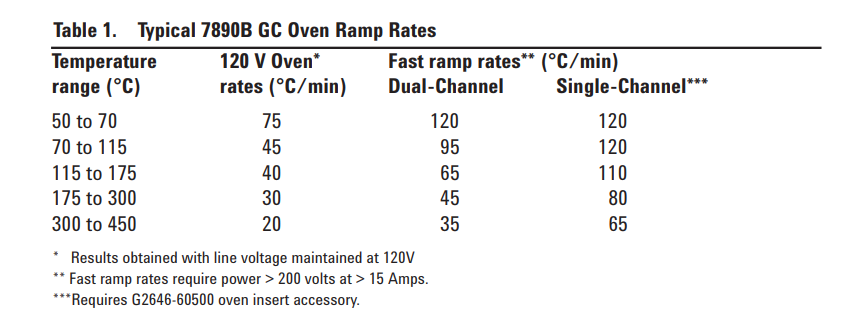
\includegraphics[width=0.8\textwidth]{Figures/7890B.png}
	\decoRule
	\caption[A temperature-rate table from the Agilent7890B data sheet]{The
	temperature-rate table from the Agilent 7890B chromatograph data sheet.
	\autocite{7890B}. }
	\label{fig:RampRate7890B}
\end{figure}

\begin{figure}
	\centering
	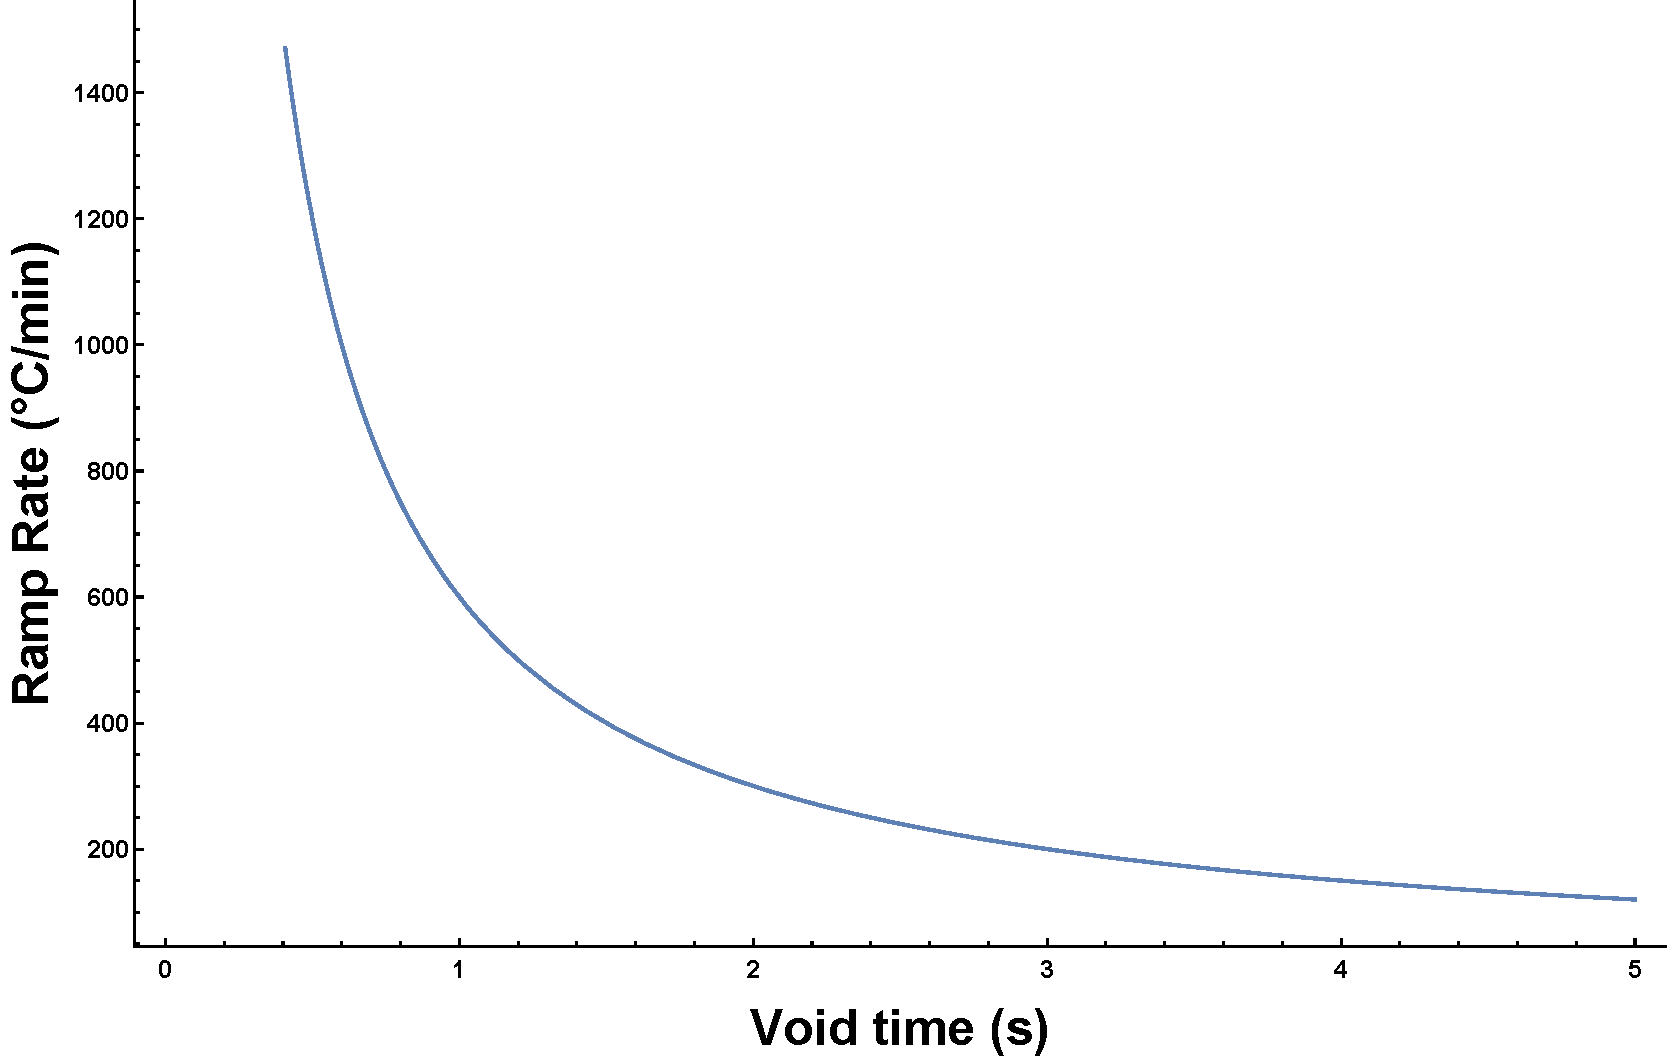
\includegraphics[width=0.8\textwidth]{Figures/RampRate.pdf}
	\decoRule
	\caption[Suggested ramp rate]{The suggested ramp rate for temperature-programmed gas chromatography as a function of void time.}
	\label{fig:RampRateBlumberg}
\end{figure}

The ramp rate of conventional air baths is limited by three factors:

\begin{itemize}
	\item The low heat capacity of air
	\item The poor thermal conductivity of air
	\item The mass of the oven that needs to be heated. 
\end{itemize}

There is very little that can be done about these matters. Attempts by
instrument manufacturers to create air baths with faster ramp rates include
decreasing the size of the oven and increasing the air flow rate, which yields
modest improvements.

\subsection{Resistive heating}

Fortunately, the heating rate problem has a technologically simple solution,
namely \keyword{resistive heating}\footnote{Alternative methods of heating by
electromagnetic fields are \keyword{radiative heating}, \keyword{inductive
heating} and \keyword{dielectric heating}.}. When a constant electric field is
applied to a metal, the free electrons in the metal will be accelerated by the
electric field. But the electrons are within the crystal lattice of the metal,
where their mean free path is very short. The electrons will therefore collide
with atoms in the crystal lattice, scattering inelastically. The energy lost in
the inelastic collisions will increase the vibrational energy of atoms, and
this energy will appear as heat.

The number of electrons and their average (drift) speed in combination is
described by a measure called the \keyword{current} (\(I\)), and the electric
field can be described by the applied \keyword{voltage} (\(V\)). The current
\(I\) is proportional to the applied voltage, and the ratio \(\frac{V}{I}\)
defines a proportionality constant \(R\), called the \keyword{resistance}, which
is a function of the conductor's material and dimensions. The total
\keyword{power} dissipated to heat (\(P\)) is given by \(P=IV\) or,
equivalently, \(P=I^2R\) or \(P=\frac{R}{V^2}\).

Applying a voltage \(V\) to a metal element close to a chromatographic column
will heat the metal, and therefore the column in contact with it. The rate at
which the piece of metal heats up depends on the power dissipated, the mass of
the metal, and its heat capacity. If the volume of the metal is small enough,
and the current high enough, the temperature of the metal element (and with it
the temperature of the column) will increase at a rate high enough to be useful
in fast chromatography. By suitable manipulation of \(V\), then, the temperature
of the column can then be changed at any desirable rate.

This technology has been reviewed \autocite{Wang2012, Jacobs2013, Miranda2010},
and a few technologies for resistive heating of capillary columns have emerged:

\begin{itemize}
  \item Direct heating of a metal column or a column coated with a metal layer
  \item Collinear heating
  \item Coaxial heating
\end{itemize}

The first SFC×GC work done \autocite{Venter2004} used a directly heated metal
column. While this approach proved the concept, experience showed two
shortcomings. Firstly, metallic columns are usually designed with specific
high-temperature applications in mind. This means that metal columns are not
available with all the stationary phases available in fused-silica columns.
Secondly, it was harder than expected to control the temperature accurately. The
temperature was determined by a thermocouple glued to the column, which was
sensitive to local variations.

An example of collinear resistive heating is Agilent\texttrademark{}'s `low
thermal mass' column, which includes collinear heating wire and a collinear
sensing element bundled with a short fused silica column. This approach requires
that the collinear heating element be wrapped in close contact with the column
as part of the manufacturing process.

For the work presented in this thesis, a coaxial heater was used. This heater is
in the form of a thin-walled stainless-steel tube that carries the electric
current. It was made of a \SI{940}{\milli\metre} length of SAE 304 stainless
steel with an outside diameter of \SI{1.06}{\milli\metre} and an inside diameter
of \SI{0.80}{\milli\metre}, obtained from Mifam (Milanówek, Poland). The column
was threaded inside the stainless steel tube, which put it in close contact with
the heater for reliable heat transfer. The coaxial heater can be coiled to
fit inside a conventional GC oven.

This coaxial design has the advantage that the column can be changed without
changing the resistive heater. This means that there is no need to re-calibrate
the heater when columns are changed.

\begin{figure}[htbp]
	\centering
	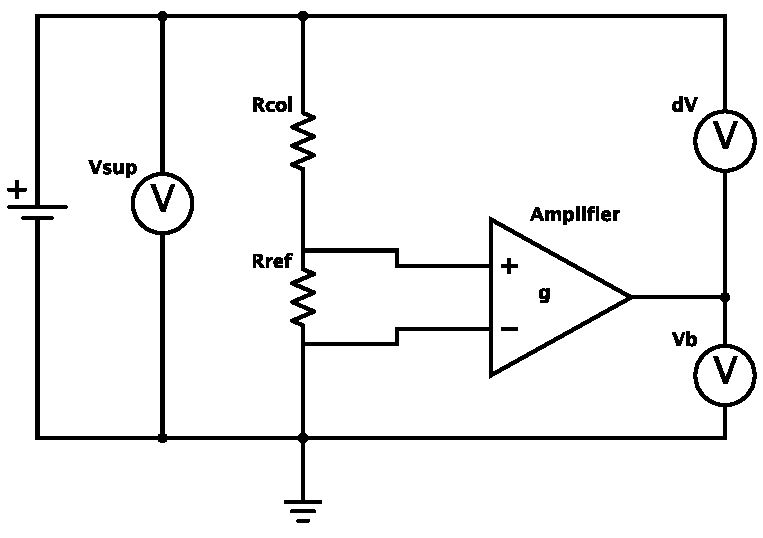
\includegraphics[width=0.8\textwidth]{Figures/Column-Heater.pdf}
	\decoRule
	\caption[Coaxial heater resistance heater]{\label{fig:HeaterDiagram}Electric circuit diagram of the coaxial heater.}
\end{figure}

The electrical resistance of a conductor is determined by its dimensions, the
material it is made of, and the temperature of that material. In a conductor of
given dimensions, therefore, a knowledge of the resistance implies a knowledge
of the temperature. By following changes in the resistance, one can determine
changes in the temperature, and by comparing resistance at certain temperatures
with known temperatures, one can get a calibrated temperature from a given
resistance.

High-powered resistive heating at safe, convenient voltages implies low
resistance. Measuring the \emph{absolute value} of low resistance is
technologically challenging \autocite{Dyos2012}. But a simple electronic circuit
can be used to \emph{compare} the resistance of the coaxial heater with that of
a reference resistor (Figure \ref{fig:HeaterDiagram}). The circuit is supplied
by a voltage \(V_{sup}\), in general an unknown value. \(V_{col}\) and
\(V_{ref}\) represent the voltage drops over the respective resistors. Because
the current \(I\) through the circuit is the same for both \(R_{col}\) and
\(R_{ref}\), it is true that \(\frac{R_{col}}{V_{col}} = \frac{ R_{ref} }{
V_{ref} }\), and therefore

\(R_{col} = R_{ref}\frac{V_{col}}{V_{ref}}\)

The voltage drop across $R_{ref}$ is too small to be directly digitized,
therefore it is amplified by an amplifier with gain $g$, so that $V_b =
gV_{ref}$. $V_b$ is measured, as is $dV$, the potential difference between the
supply and the amplifier output. We can show that the coaxial heater resistance
\(R_{col}\) is a function of the voltage ratio \(\frac{dV}{V_b}\).

First, 
\[ V_{sup} = V_{col} + V_{ref} \] 
but also
\[ V_{sup} = dV + V_b \]
Therefore,
\[ V_{col} + V_{ref} = dV + V_b \]
But \(V_{b} = g V_{ref}\), so
\[ V_{col} + V_{ref} = dV + gV_{ref} \]

\[ V_{col} = dV + gV_{ref} - V_{ref} \]

\[ V_{col} = dV + V_{ref}(g - 1) \]

\[ \frac{\displaystyle V_{col}}{\displaystyle gV_{ref}} = dV/gV_{ref} + V_{ref}(g-1)/gV_{ref} \]

\[\frac{\displaystyle V_{col}}{\displaystyle V_{ref}} = gdV/gV_{ref} + gV_{ref}(g-1)/gV_{ref} \]

\[\frac{\displaystyle V_{col}}{\displaystyle V_{ref}} = g\frac{dV}{V_b} + (g-1) \]

This proves that \( \frac{\displaystyle V_{col}}{\displaystyle V_{ref}} \) is a
linear function of $dV/V_b$. A quick check for correctness of the expression:
for a unity-gain amplifier $g = 1$, and $\frac{\displaystyle
V_{col}}{\displaystyle V_{ref}} = dV/V_b$.

Therefore 

\[ R_{col} = R_{ref} \left(\frac{g{dV}}{V_b} + (g-1) \right) \]

In practice the gain \(g\) is not completely constant, but shows a slight
dependence on \(dV\), so a general expression might be

\[ R_{col} = f\left(\frac{dV}{V_b} \right) \]


\section{Calibration}

The assumption is that the temperature is a function of the resistance of the
coaxial heater, or \( T = g(R_{col}) \). Because \( R_{col}=f(\frac{dV}{V_b}) \),
we can see that \( T = g(f(\frac{dV}{V_b})) \), or, because a function \(g\) of
a function \(f\) is a function \(h\) (\(f \circ g = h \)), \( T =
h(\frac{dV}{V_b}) \).  Through a calibration procedure \(h\) can be
approximated by a polynomial or lookup table.

\subsection{Temperature uniformity}
\label{sec:Uniformity}

It is highly desirable that the coaxial heater should give uniform heating, but
there is no obvious guarantee an electrically heated tube will heat uniformly.
We did not analyse the problem theoretically, but the following factors will
play a role:

\subsubsection{Resistivity's dependence on temperature}

The resistance of a metal increases with temperature. This means that if one
section of the coaxial heater gets hotter than the rest, its resistance
will increase. If the current were to remain constant, more power would be
dissipated in this section (\(P=I^2R\)). If more power is dissipated, the
temperature will increase, leading to a higher resistivity, leading to higher
power dissipation, leading to a higher temperature, in a runaway cycle. In
contrast, if the coaxial heater was made of a material of which the resistivity
decreases with an increase in temperature, the temperature along the length of
the heater would be stabilized by negative feedback. In the case of the supply
voltage being held constant a higher resistance in one section would mean a
lower current overall, but still a higher power dissipation in the section with
higher temperature.

\subsubsection{Thermal conduction}

Each section of the coaxial heater is in thermal contact with its neighbours. If
it were to get hotter, the heat will flow from the hotter section to the cooler
neighbouring sections. This will tend to even out any temperature differences.
This longitudinal equilibrium process is inefficient for a long, thin-walled
tube.

\subsubsection{Radiation}

An object radiates heat, which can be approximated by the Stefan-Boltzman law:

\begin{equation}\label{eq:1}
	P=A \epsilon \sigma T^4
\end{equation}

where A is the surface area of the object, \(\epsilon\) is the
\keyword{emissivity} of the surface, \(\sigma\) is the Stefan-Boltzman constant,
and \(T\) is the absolute temperature of the object. 

If a section of the coaxial heater were to become hotter than the other
sections, it would therefore radiate more heat. The increased power dissipation
by the higher resistance will therefore be partially offset by a higher
radiation. This will tend to moderate temperature differences.

\subsubsection{Convection}

When a part of the coaxial heater is hot, it will heat the air around it through
radiation and conduction. This air might then move, through buoyancy or any
other force, past another part of the coaxial heater. This second part could
then be heated up by the transported air. For example, a vertically mounted
coaxial heater can be expected to develop a temperature gradient from bottom to
top, as natural convection lets hot air transfer heat from the lower end of the
heater to the upper end. In this way temperature gradients could be established
and maintained.

\subsubsection{Examining thermal uniformity by imaging}

The effect of the combination of resistivity's temperature dependence, thermal
conduction, radiation, and convection on the temperature uniformity of the
coaxial heater could be mathematically or numerically modelled, but such an
endeavour would fall outside the scope of this project. Experience had not led
us to expect any significant temperature non-uniformity, but we welcomed the 
opportunity to get empirical confirmation.

\keyword{Thermal imaging} is the process by which infrared radiation from
objects can be captured in a photographic process. At near-ambient temperatures
objects emit copious amounts of infrared radiation, and the higher the
temperature, the more is emitted. (See Equation \ref{eq:1}.) Cameras designed
using specialized optics and sensors allow the capture of that radiation as an
image of a scene that shows objects based on their surface temperature. The
technological capability of thermal imaging has improved markedly over the past
years.

Using a FLIR{\texttrademark} T660 thermal imaging camera we obtained a video of
the coaxial heater executing three consecutive temperature ramps. This camera
uses a \num{640 x 480} focal plane uncooled bolometer array as a detector, which
is sensitive to radiation in the range \SI{7.5}{\micro\metre} to
\SI{14}{\micro\metre}. Figure \ref{fig:ThermalImageSetup} shows the setup used
to record the thermal video. To get reliable temperature information from a
thermal image requires calibration or a precise knowledge of the material's
\keyword{emissivity}. In the absence of such calibration, the obtained
temperature measurement is more useful if seen as relative rather than absolute.

\begin{figure}
	\centering
	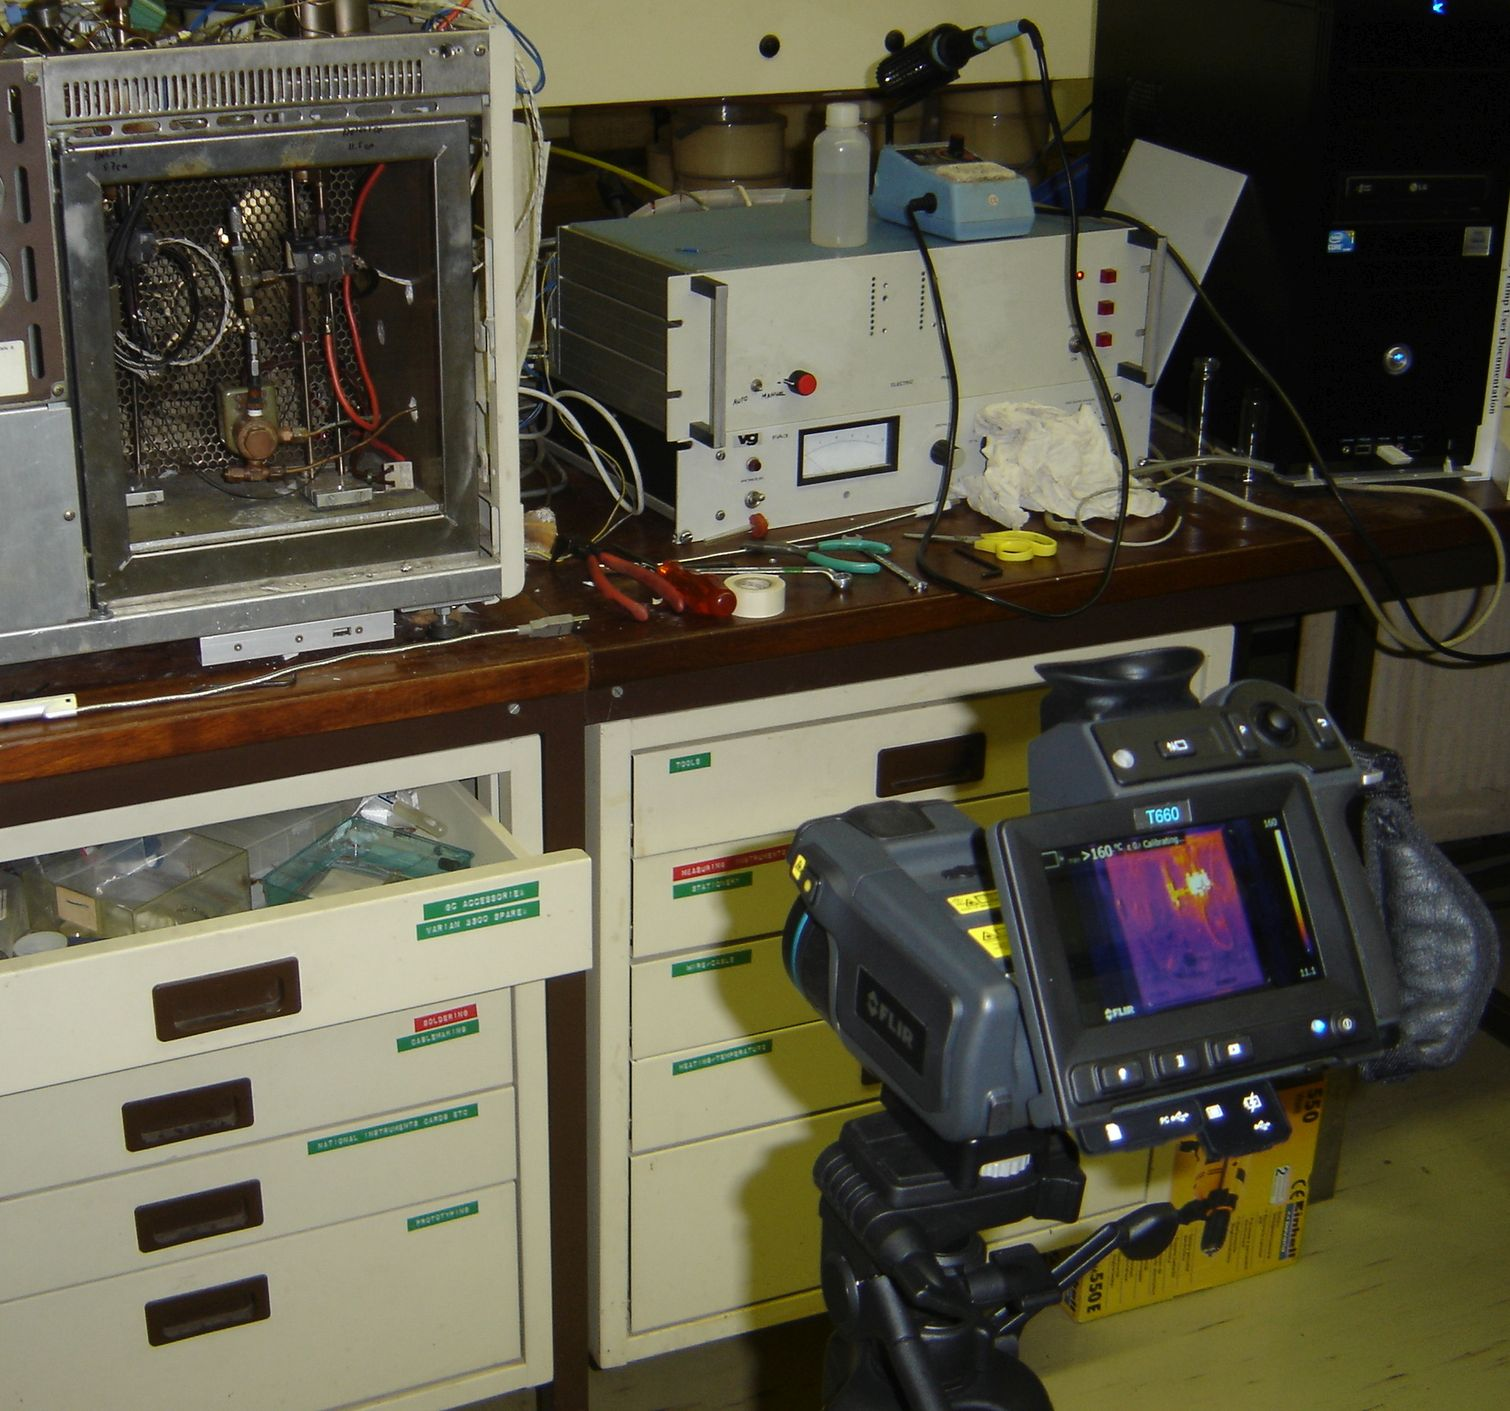
\includegraphics[width=0.8\textwidth]{Figures/ThermalImageSetup}
	\decoRule
	
\caption[A photograph of the setup used to record the thermal video]{This
photograph shows the setup used to record the thermal video.}
	
	\label{fig:ThermalImageSetup}
\end{figure}

The video showed that the three consecutive temperature runs heated the coaxial
heater identically. Figure \ref{fig:ThermalImage} is a frame from the video,
analysed to give estimates of the temperatures on spots on the coaxial heater.
The maximum temperature difference between any two points is
\SI{17.5}{\celsius}, and there are no marked gradients.

\begin{figure}
	\centering
	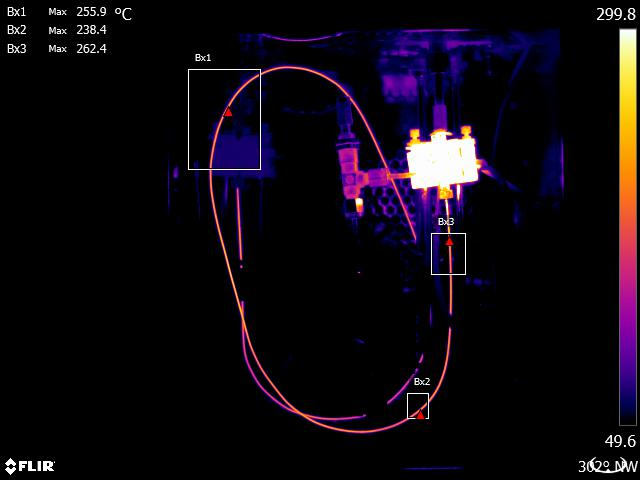
\includegraphics[width=0.8\textwidth]{Figures/ThermalImage}
	\decoRule
	
\caption[A thermograph of the coaxial heater at temperature]{A thermograph of
the coaxial heater at high temperature. It shows that there are no runaway hot
spots.}
	
	\label{fig:ThermalImage}
\end{figure}

This examination of the uniformity of the coaxial heater helped to dispel fears
that unexpected temperature gradients would interfere with the fast gas
chromatography. 

\subsection{Temperature calibration}

When doing temperature-programmed gas chromatography it is desirable to have an
absolute measurement of the column temperatures. This makes it possible to
translate and compare methods between instruments. It was therefore necessary to
calibrate the temperature of the coaxial heater. Calibration is the comparison
of measurement values from a device under test with those of a calibration
standard of known accuracy. In the case of the temperature calibration of the
coaxial heater, it means comparing the results of the temperature as measured by
the coaxial heater with a standard temperature.

The problems of measuring a temperature inside a tube with a bore of
\SI{0.8}{\milli\metre} are not trivial, and to solve them we examined the
available technologies to find the optimum solution.

The following temperature measurement technologies exist:
\begin{itemize}
	\item Liquid-in-glass thermometers
	\item Sealed liquid or gas sensing instruments and bimetallic sensors
	\item Electrical resistance temperature measurement using metallic sensors
	\item Thermistors and semiconductors
	\item Thermoelectric temperature measurement
	\item Disappearing filament optical pyrometer
	\item Photoelectric optical pyrometers
	\item Total radiation pyrometers
\end{itemize}

Liquid-in-glass thermometry would not be applicable because of the size of the
devices, and because they don't give a desirable electrical signal. Bimetallic
and sealed liquid or gas sensing elements are also too bulky and are best used
where only an on/off electric signal is required.

In recent years \keyword{pyrometry}, the technology of measuring temperature by
radiant energy methods, have improved markedly and has become affordable, in the
form of thermal cameras. However, at lower temperatures the accuracy of the
recorded temperature depends heavily on the emissivity of the measured material.
Thermal imaging will also only measure the outside wall surface temperature of
the heater, and not the temperature on the inside of the coaxial heater. So,
while thermal imaging settled questions about heater uniformity (Section
\ref{sec:Uniformity}), it was not considered ready to serve as a calibration
standard.

The remaining options are resistance temperature measurement with metallic sensors,
thermistors and semiconductors, and thermoelectric temperature measurement.

Electrical resistance measurement using metallic sensors might have been
feasible, if sensing elements of the appropriate dimensions were commercially
available. A further difficulty with this method of temperature measurement is
that long, thin conductors would be needed to connect the sensing element to the
electronics. These conductors would add to the resistance measured by the
sensing element, requiring complex correction or multi-wire measuring methods.

Thermistor and semiconductor devices could be made small enough, but all
commercially available packages are too large. Besides, the temperature range
used in GC (\SI{-50}{\celsius} to \SI{400}{\celsius}) does not fall inside the
operating temperature range specified by manufacturers of semiconductor devices
(\SI{-55}{\celsius} to \SI{125}{\celsius} for military applications)
\autocite{nullD1996}.

Thermoelectric temperature measurement was the only remaining alternative, and
was used to calibrate the coaxial heater. In particular, the \keyword{Seebeck
effect} was exploited, which is the observation that a temperature gradient
imposed on a metallic conductor will generate an electrical potential along the
gradient. Therefore, a circuit of two dissimilar metallic conductors will
generate a voltage when there is a temperature gradient along the conductors.
The voltage generated is a function of the temperature difference between the
hot junction of the two metals and their cold junctions at the voltmeter input.
Such a pair of dissimilar conductors used to generate a voltage is known as a
\keyword{thermocouple}, and this technology is mature and widely used in
industry. Standard thermocouples are constructed from well-characterized alloys
that generate predictable voltages for given junction temperatures. Pairs of
thermocouple standardized alloys are known as 'types', of which the
general-purpose Type K suited our purpose best. Thermocouple wire can be
purchased in a range of gauges, down to \SI{25}{\micro\metre} in diameter, and
the signal processing for thermocouple signals have been standardized.
Thermocouple junctions can be made by welding, crimping, soft soldering, hard
soldering, bolting, or simply twisting the wires together \autocite{McGee1988}.
Because the temperature range to be measured was ({-}50 \si{\celsius} to 400
\si{\celsius}) soft soldering is not a viable choice, because soft solders have
melting points around \SI{200}{\celsius}. The possibility of corrosion and
mechanical vibration suggests that twisting the wires together will not form a
reliable joint, and of course there are no sub-millimetre bolts on the market.

This leaves welding, crimping and hard soldering as methods for making
thermocouple junctions. Tools for crimping hair-fine wire are rare and it is
likely that a practical crimped connection will have a diameter many times the
diameter of the wire, possibly making it too large to fit.

Hard soldering is usually done with a high-temperature flame, and on contact the
flame will rapidly burn the fine wires and destroy them. The temperature
required for hard soldering is still lower than the melting point of the wires,
so that hard soldering is not excluded, but we did not have the knowledge or the
technology to solve the associated problems.

Welding was found to be an accessible technology for forming small, reliable
joints in fine thermocouple wire.

\subsection{Thermocouple welding}

Welding is the process of joining two metal parts by melting a portion of each
part, allowing the molten metals first to mix, and then to solidify. This
creates a permanent joint between the two metals. Welding is widely practised as
an industrial process in applications ranging from shipbuilding to
microelectronics. Previous work in our laboratories used capacitive discharge
spot welding to melt the spot where two wires crossed. These thermocouples were
found to be too fragile for the intended application, so a method was developed
to yielded a more robust thermocouple.

In the laboratory, electricity is the most convenient source of heat. A
\SI{24}{\volt} direct current, adjustable bench power supply was used to supply
the current. The two wires of the thermocouple were twisted together and the
twisted pair was connected to one pole of the power supply. A carbon electrode
was connected to the other pole. The carbon electrode was carefully brought
closer to the thermocouple pair until a spark jumped across the air gap. When
the spark turned into an arc the heat of the arc melted the end of the twisted
pair. The molten metal would then contract into a spherical globule, which grew
as the arc added more heat. As more of the metal of the wire melted, the globule
would move away from the carbon electrode, until the gap became too large to
sustain the arc. The current would then stop, leaving a spherical welded bead at
the end of the wires. (See Figure \ref{fig:WeldingSteps}.) The process could be
repeated as often as necessary to obtain a bead of the desired size.

It is worth noting that it is necessary to form an arc: if the carbon electrode
happens to touch the wire so that a current flows directly from the wire to the
carbon electrode the wire rapidly heats up over its length and melts. It is also
seems necessary to have a roughly broken carbon electrode surface: a polished
surface would not generate an arc, or even make electrical contact with the
wires. This might be because the graphite used for the electrode was formulated
for use in pencils.

The apparatus used to do the welding is depicted in Figure
\ref{fig:FineWireWelder}, and Figure \ref{fig:TCWeldMicro} shows the image seen
through the microscope during welding.

\begin{figure}
	\centering
	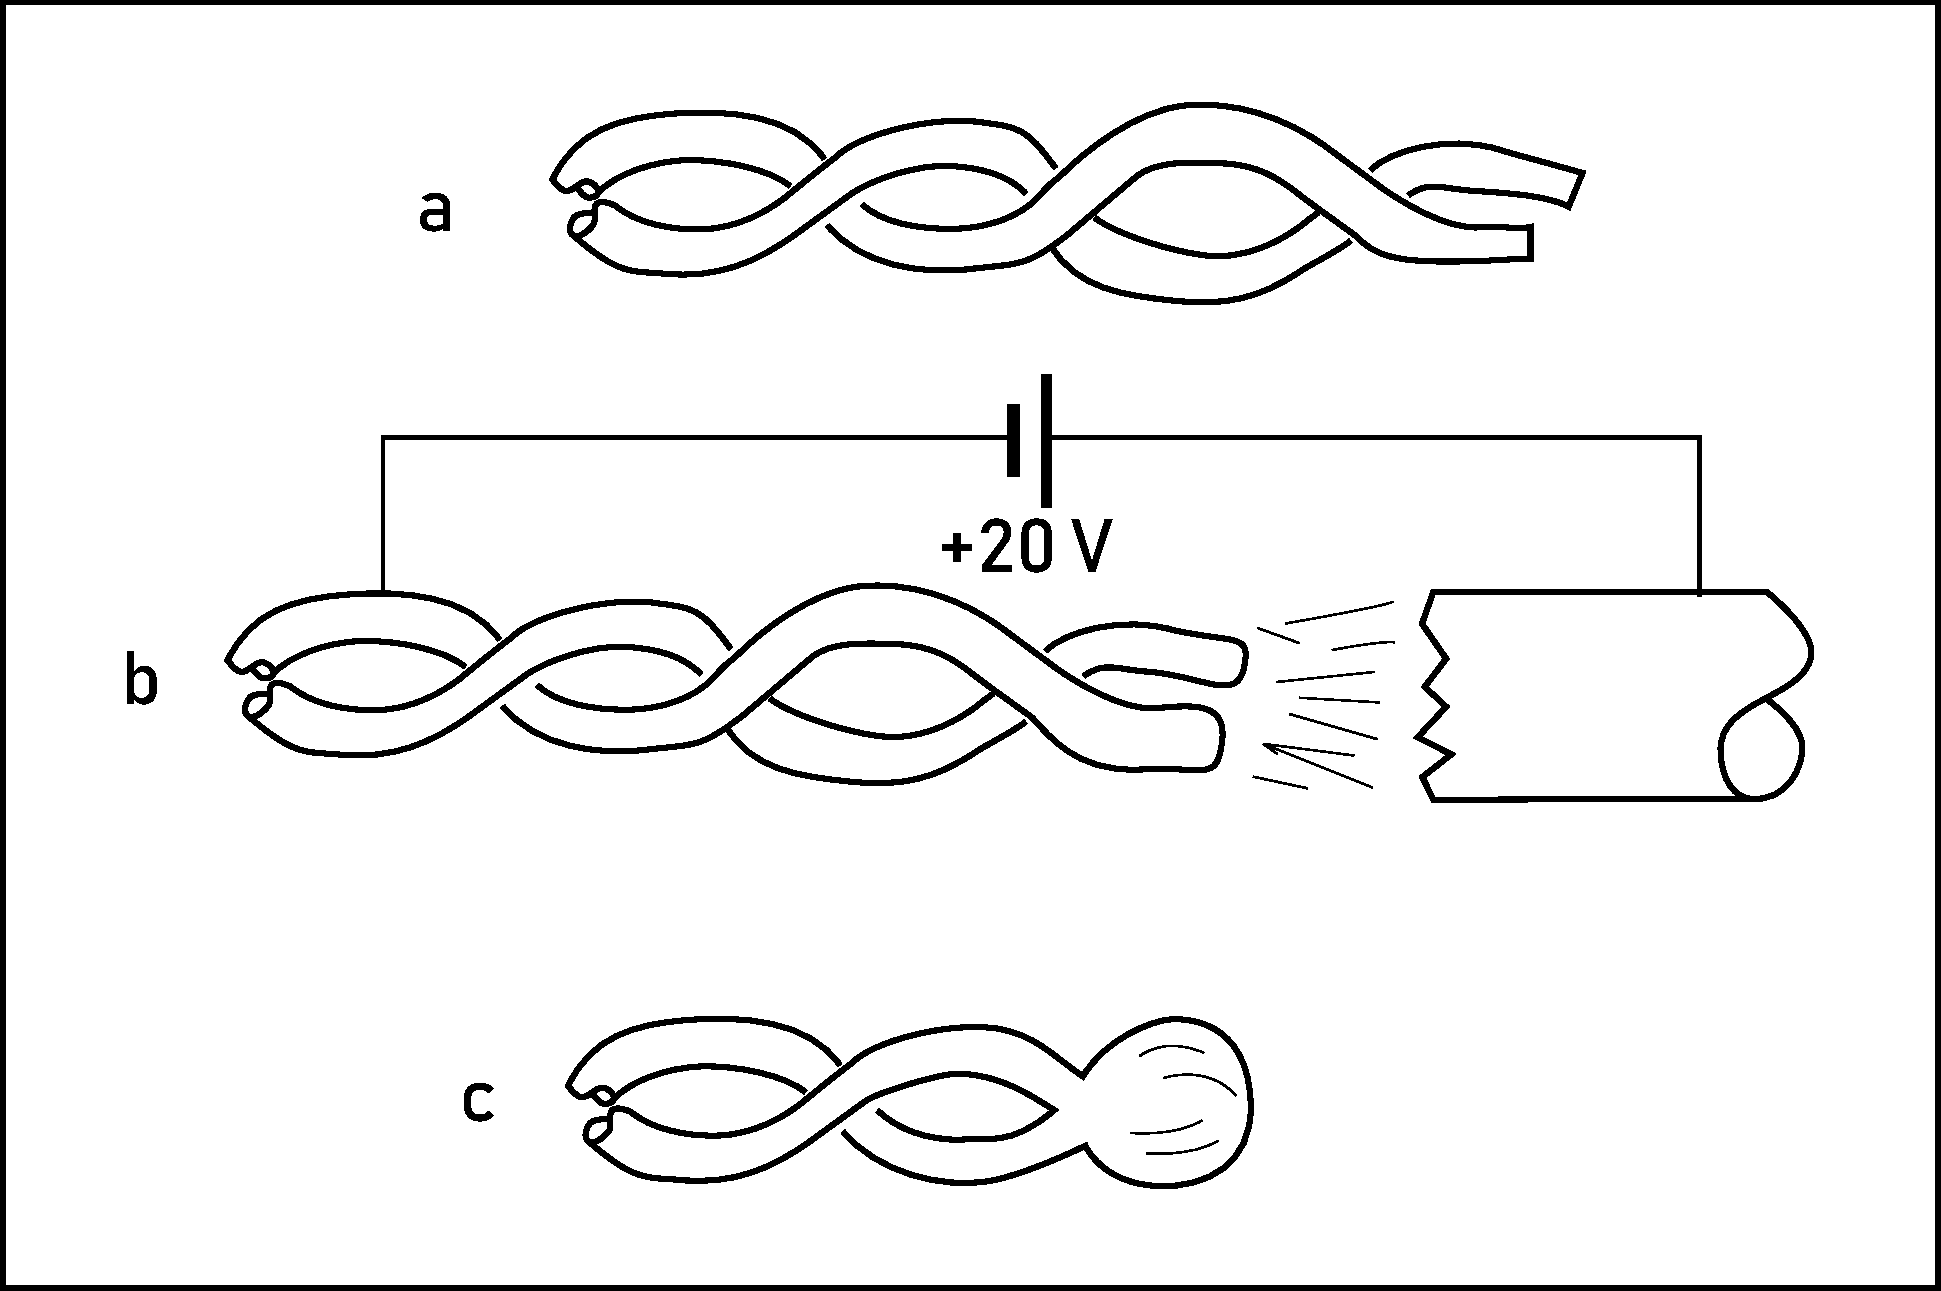
\includegraphics[width=0.8\textwidth]{Figures/TCWelding}
	\decoRule

\caption[Welding process schematic]{The process of welding fine wires to make
thermocouples (a) Wires twisted together (b) Electric arc heating up the wires
(c) Wires welded with a well-formed bead. }

\label{fig:WeldingSteps}
\end{figure}


\begin{figure}
	\centering
	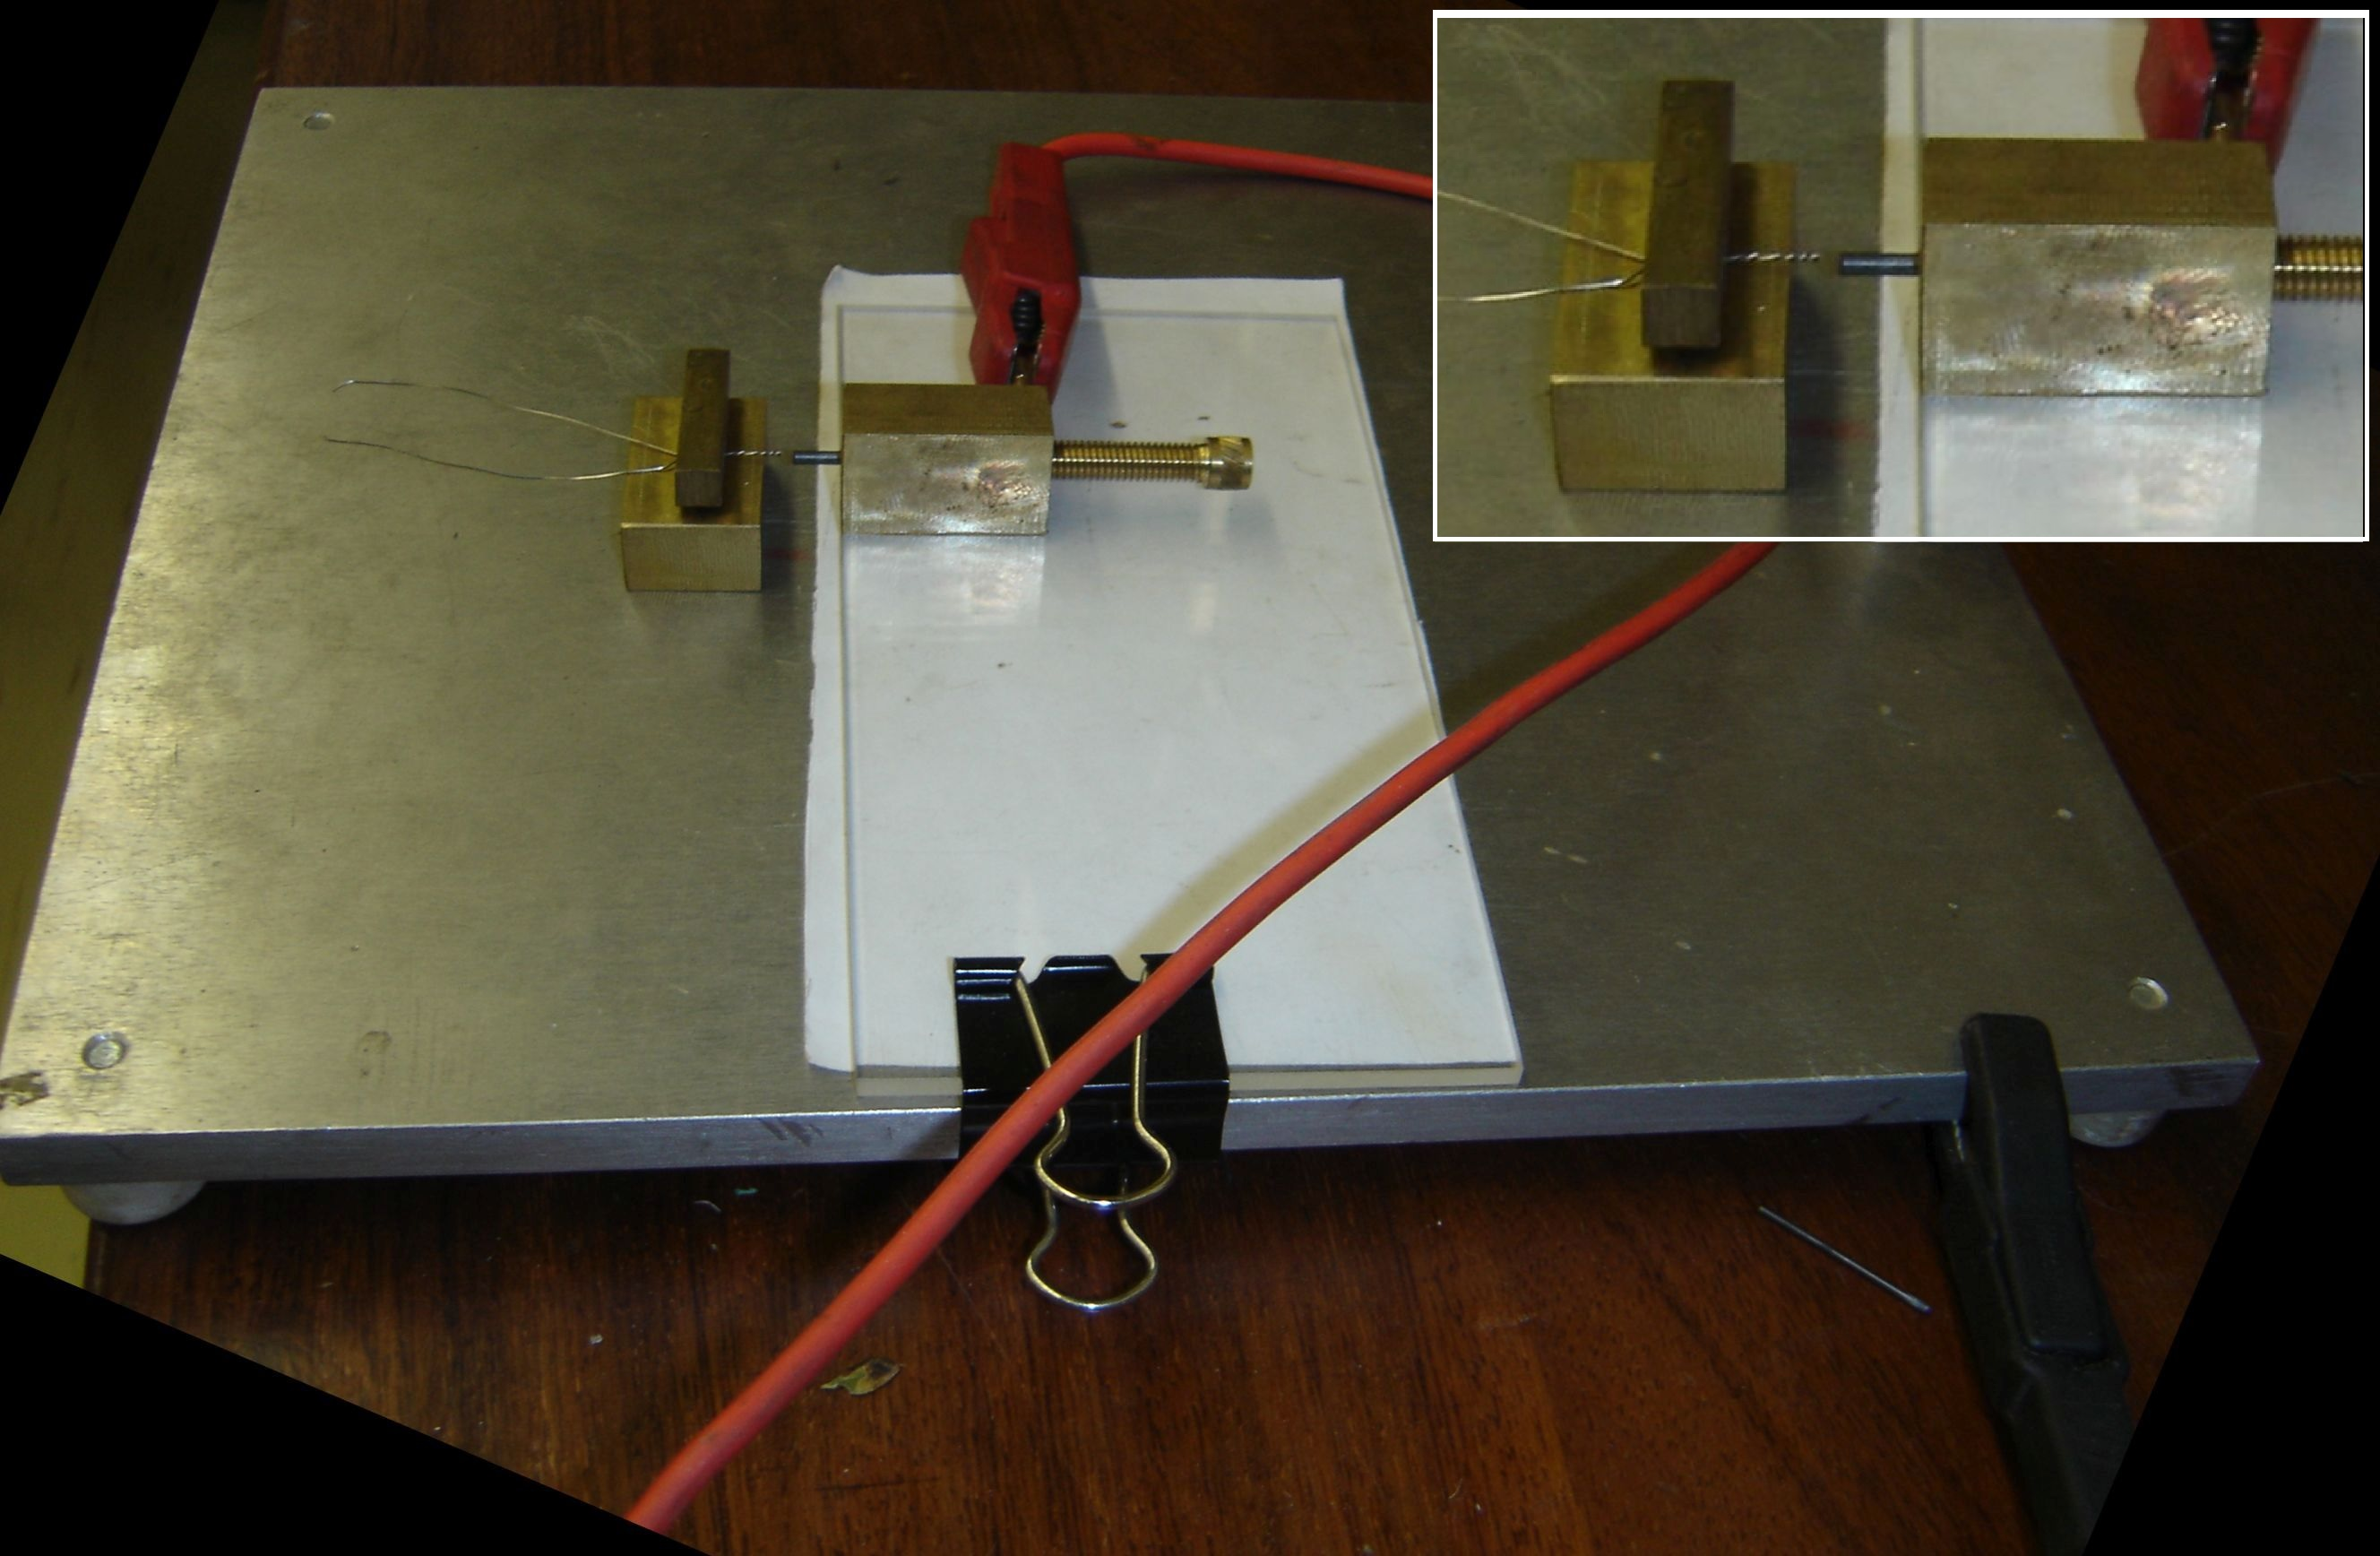
\includegraphics[width=0.8\textwidth]{Figures/Welder3.jpg}
	\decoRule

\caption[Fine-wire welder]{A view of the fine-wire thermocouple welder, as set
up on a microscope base plate. The wire shown in the photograph is much thicker
the one actually used. It is shown clamped between the clamping bar and the
clamping weight. A thin sheet of acrylic serves to isolate the positive
electrode from the negative base. The carbon electrode can be advanced towards
the thermocouple twist using the screw. The black clamp at the bottom right-hand
corner attached to the base plate and the red clamp attached to the screw
housing provide a potential difference of approximately \SI{20}{V} between the
carbon electrode and the thermocouple. \todo{Maybe add labels}}

\label{fig:FineWireWelder}
\end{figure}

\begin{figure}
	\centering
	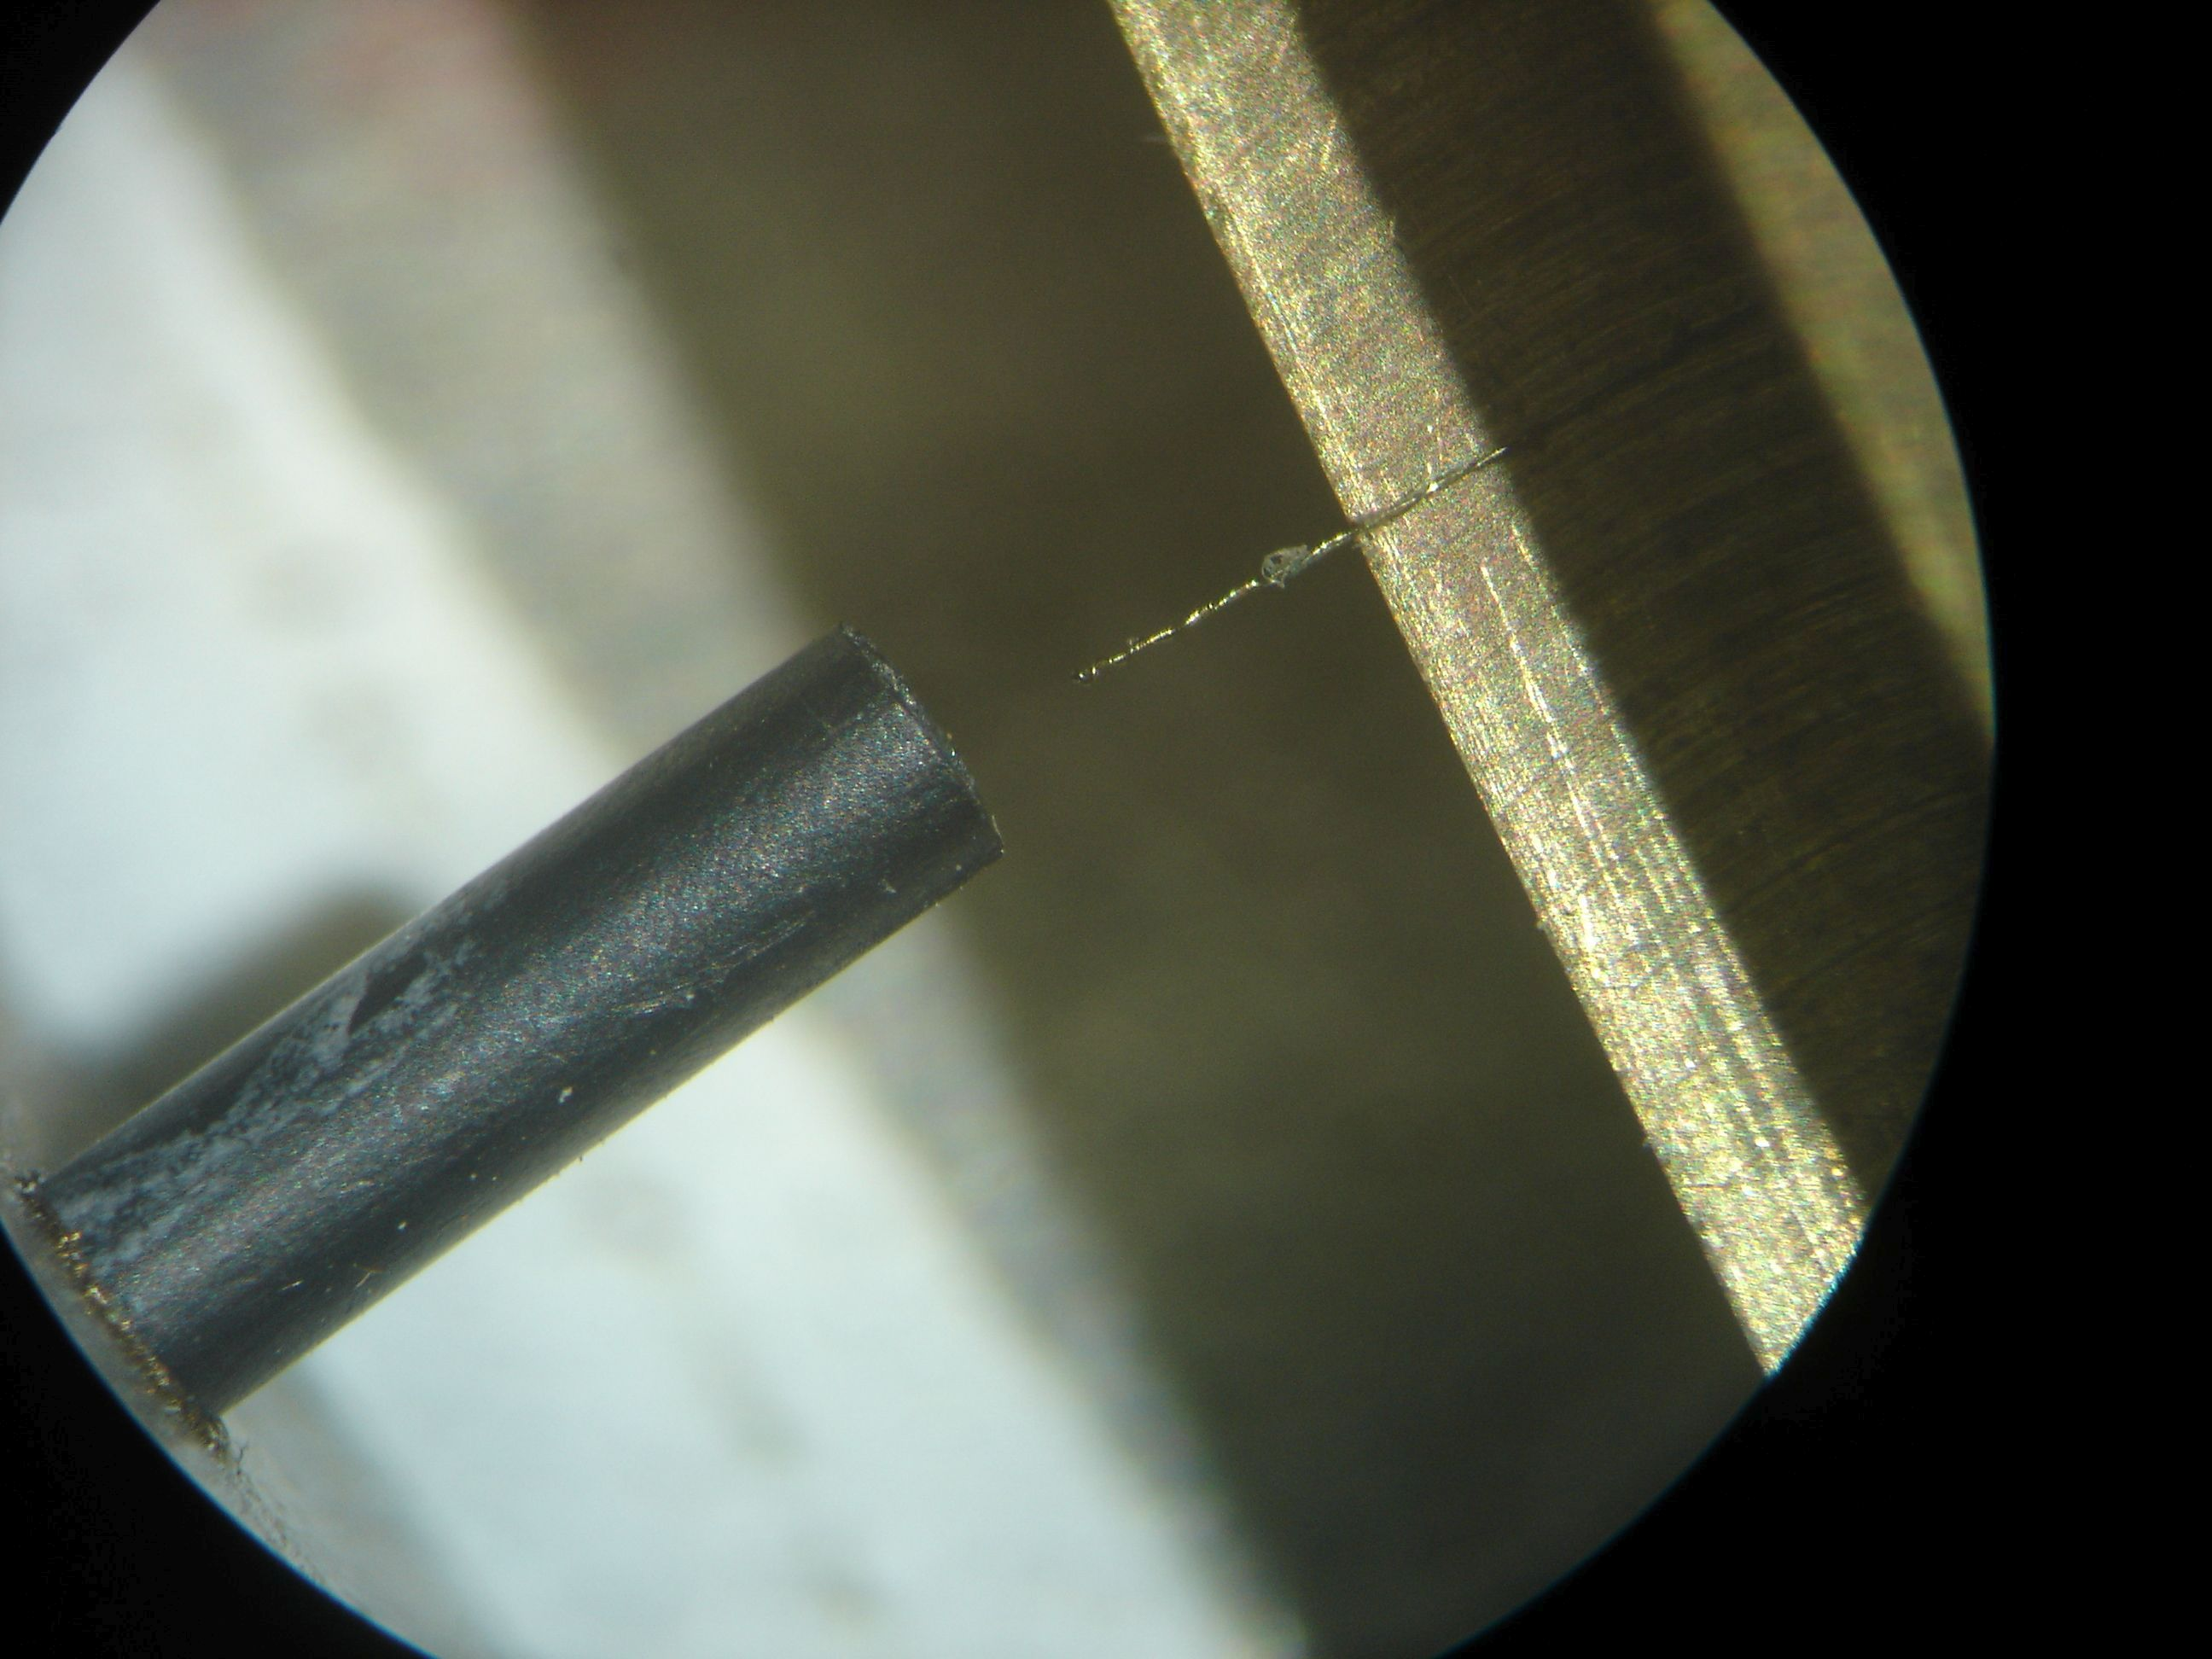
\includegraphics[width=0.5\textwidth]{Figures/WelderMicro.jpg}
	\decoRule
	
\caption[A microphoto of a thermocouple twist ready to be welded.]{A microphoto
of a pair of twisted thermocouple wires ready to be welded. The black carbon
electrode is \SI{2}{\milli\metre} in diameter.}
	
	\label{fig:TCWeldMicro}
\end{figure}

\subsection{Thermocouple probe construction}

To measure the temperature inside the coaxial heater required the thermocouple
to be inserted into the coaxial heater. For this a fused silica capillary with
an inside diameter of \SI{0.25}{\milli\metre} and an outside diameter of
\SI{0.4}{\milli\metre} was used to construct a probe. (These capillaries were
readily available, in the form of discarded chromatographic columns.) A narrower
capillary was used to draw the wires through the probe capillary, in a process
described in Figure \ref{fig:FineWireThermocouple}. The wires could then be
welded to form a thermocouple and positioned at the desired position in the
probe capillary.

\begin{figure}
	\centering
	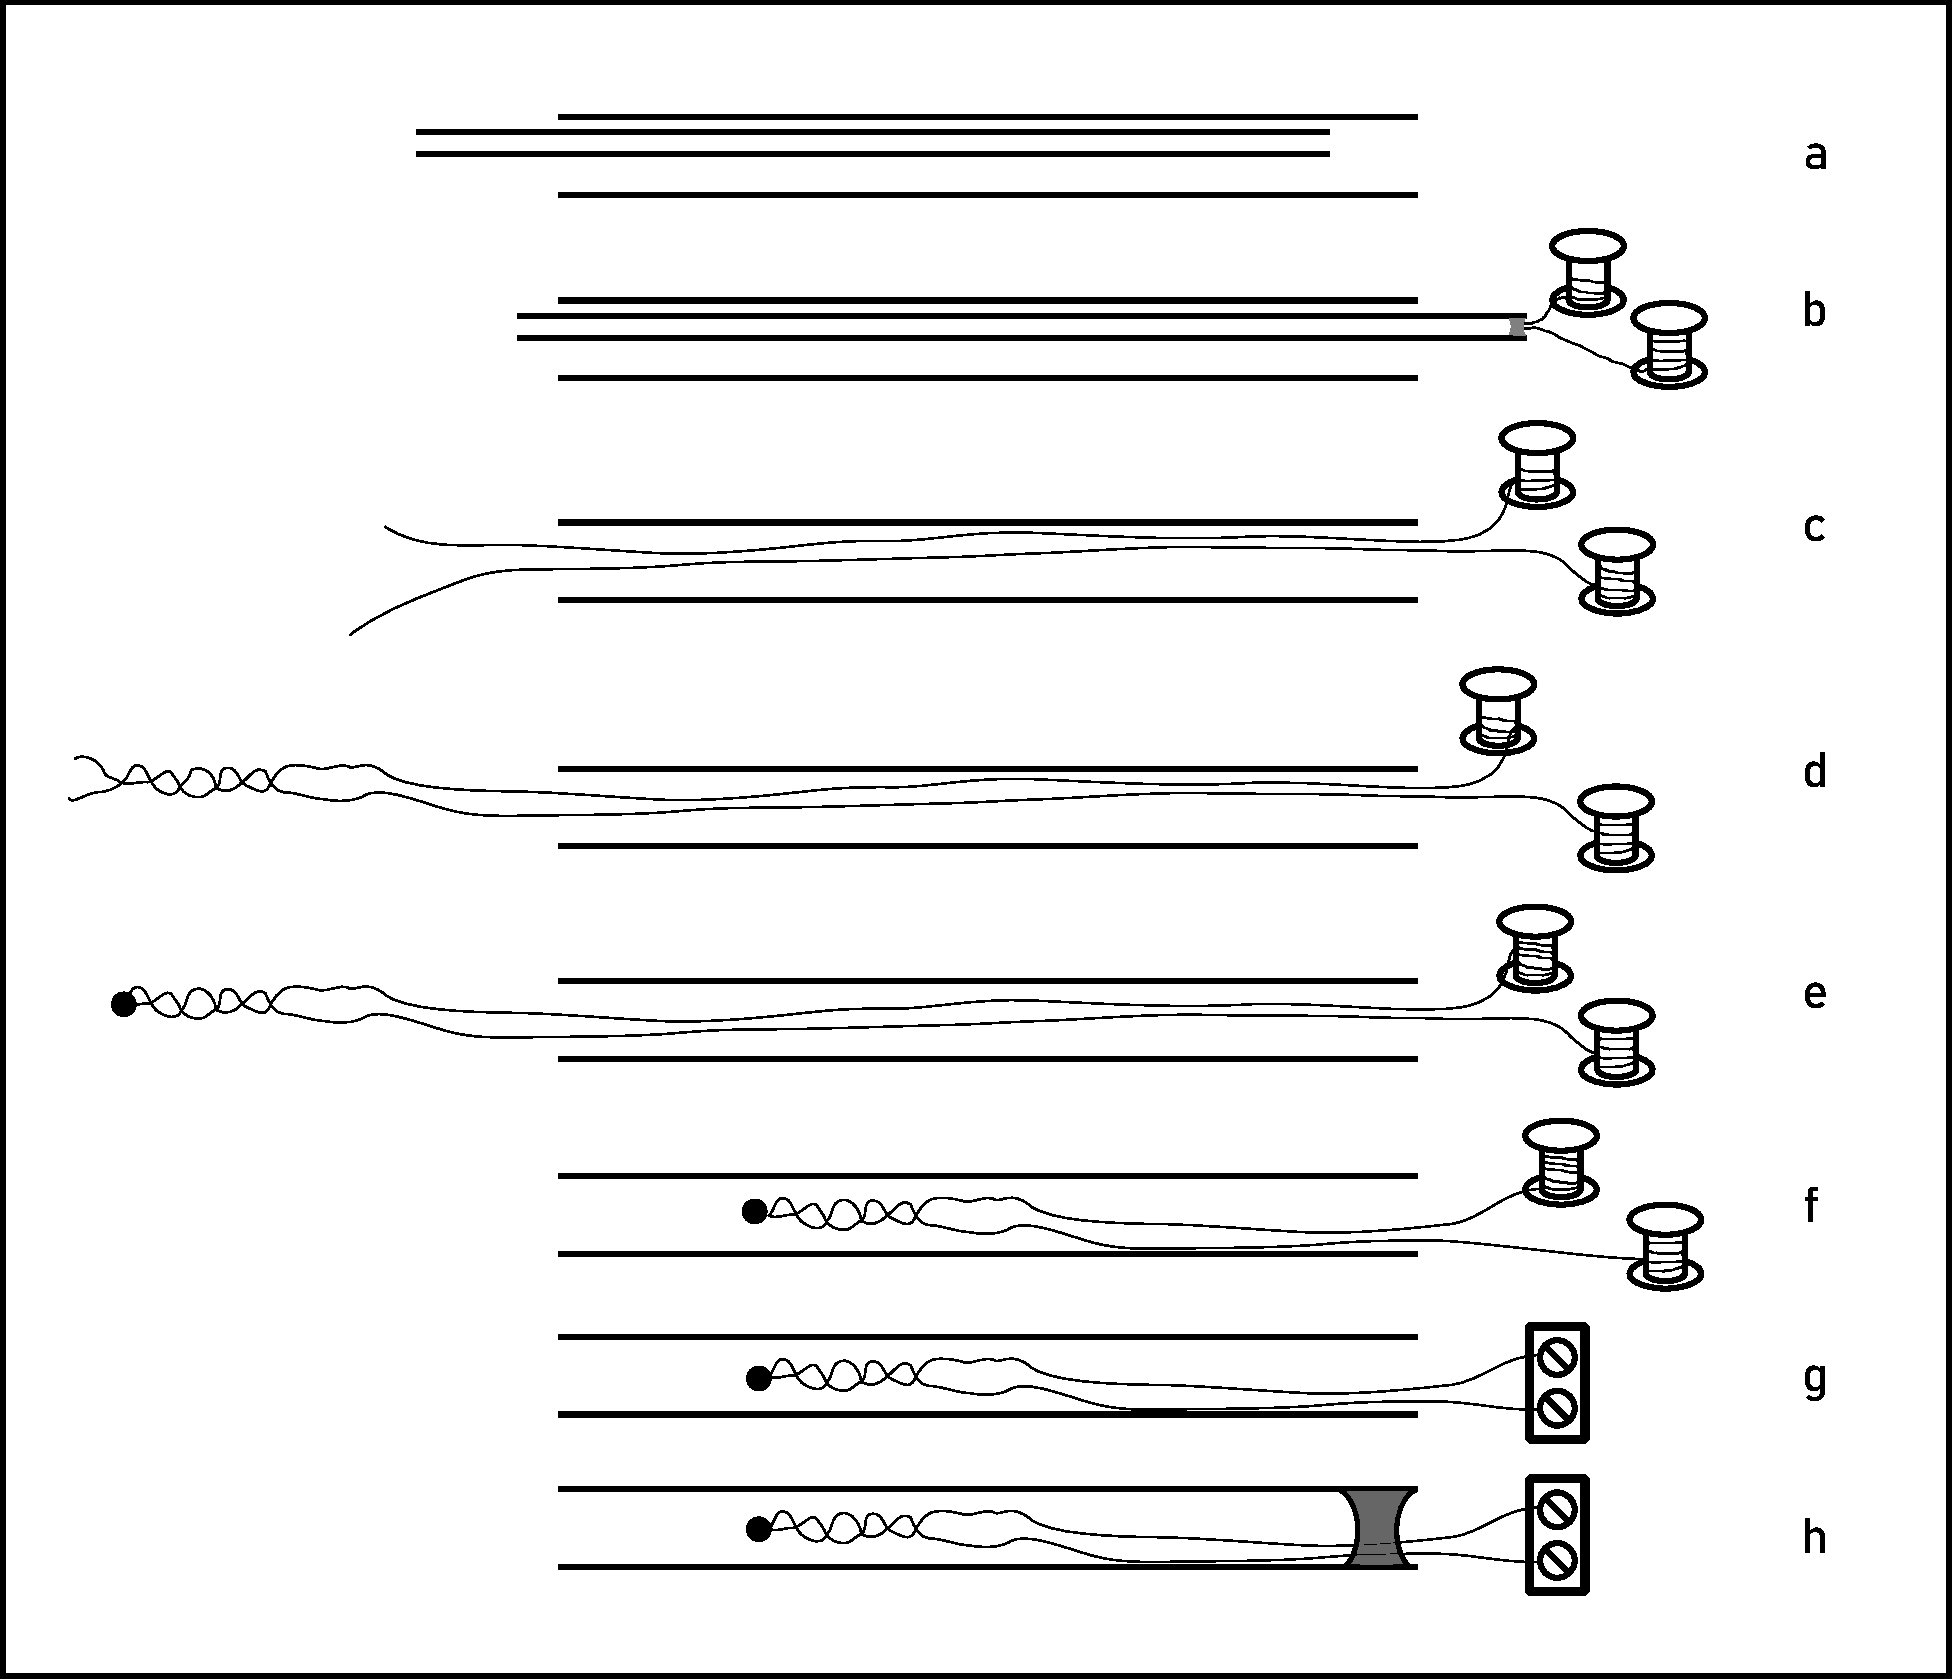
\includegraphics[width=0.8\textwidth]{Figures/FineWireThermocouple.pdf}
	\decoRule
	
\caption[A cartoon explaining how to construct a long, thin thermocouple
probe.]{(a) A narrow capillary is threaded inside a wider one (b) The ends of a
pair of thermocouple wires are fitted inside the end of the narrow capillary and
anchored with cyanoacrylate adhesive. (c) The wires are pulled through the
wider capillary using the narrow capillary. (d) The ends of the wires are twisted
together, creating a mutual mechanical anchor.
(e) The ends of the wires are welded together. (f) The wires are pulled back
into the thick capillary, locating the junction at the desired position in the
capillary. (g) The wires are trimmed and connected to a terminal block. (h) A
drop of cyanoacrylate adhesive is used to anchor the wires permanently in the
capillary. }
	
	\label{fig:FineWireThermocouple}
\end{figure}

\subsection{Thermocouple interfacing}

The Type K thermocouple has a sensitivity of approximately
\SI{41}{\micro\volt\per\celsius}. This means the voltage generated at the
temperature range of interest is too small to be conveniently digitized and
therefore must be amplified. Because the Type K thermocouple is so commonly used
in industry, amplifiers have been developed specifically for thermocouple signal
conditioning. We chose the AD595 integrated circuit amplifier. The component's
data sheet explains its application concisely: ``The AD595 is a complete
instrumentation amplifier and thermocouple cold junction compensator on a
monolithic chip. It combines an ice point reference with a pre-calibrated
amplifier to produce a high level (10 mV/°C) output directly from a thermocouple
signal'' \autocite{AD595}. The output signal of the AD595 can be directly
digitized for computer recording.

\subsection{Calibration procedure}
\label{sec:Calibration}

The International Vocabulary of Metrology \autocite{JCGM200:2012} define
\keyword{calibration} as ``[an] operation that, under specified conditions, in a
first step, establishes a relation between the \textbf{quantity values} with
\textbf{measurement uncertainties} provided by \textbf{measurement standards}
and corresponding \textbf{indications} with associated measurement uncertainties
and, in a second step, uses this information to establish a relation for
obtaining a \textbf{measurement result} from an indication.''

In the first step of calibration, the \textbf{quantity values} used in the
calibration were the temperature value of the thermocouple probe as provided by
the thermocouple voltage, the AD595 amplifier, the digitization and the
subsequent calculations according to the AD595 data sheet. The
\textbf{measurement standards} were the known responses of the thermocouple
\autocite{Ripple1995}, the amplifier and the digitization system. The
\textbf{indication} was the voltage ratio \(\frac{dV}{Vb}\). As this was a first
attempt at calibration, \textbf{measurement uncertainties} were assumed to be
negligible.

In preparation for calibration the coaxial heater was installed in the oven of
the Varian 3300 GC as it would be when in use. The detector was removed and the
thermocouple probe was threaded through the detector stem, through the heated
T-piece block, and into the coaxial heater until the thermocouple junction was
about half-way between the inlet end and the detector end of the coaxial heater.
When the system was set up as it would be during use, the coaxial heater was
cooled down before a power ramp was applied. As the power increased the
temperature rose, and the temperature of the thermocouple was recorded together
with the voltages \(dV\) and \(Vb\). A curve could then be plotted of
thermocouple temperature \(T_{TC}\) against the voltage ratio \( \frac{dV}{V_b}
\) (Figure \ref{fig:CalibrationCurve}). This revealed the shape of the function
\(T(\frac{dV}{Vb})\) and completed the first step of the calibration.

\begin{figure}
	\centering
	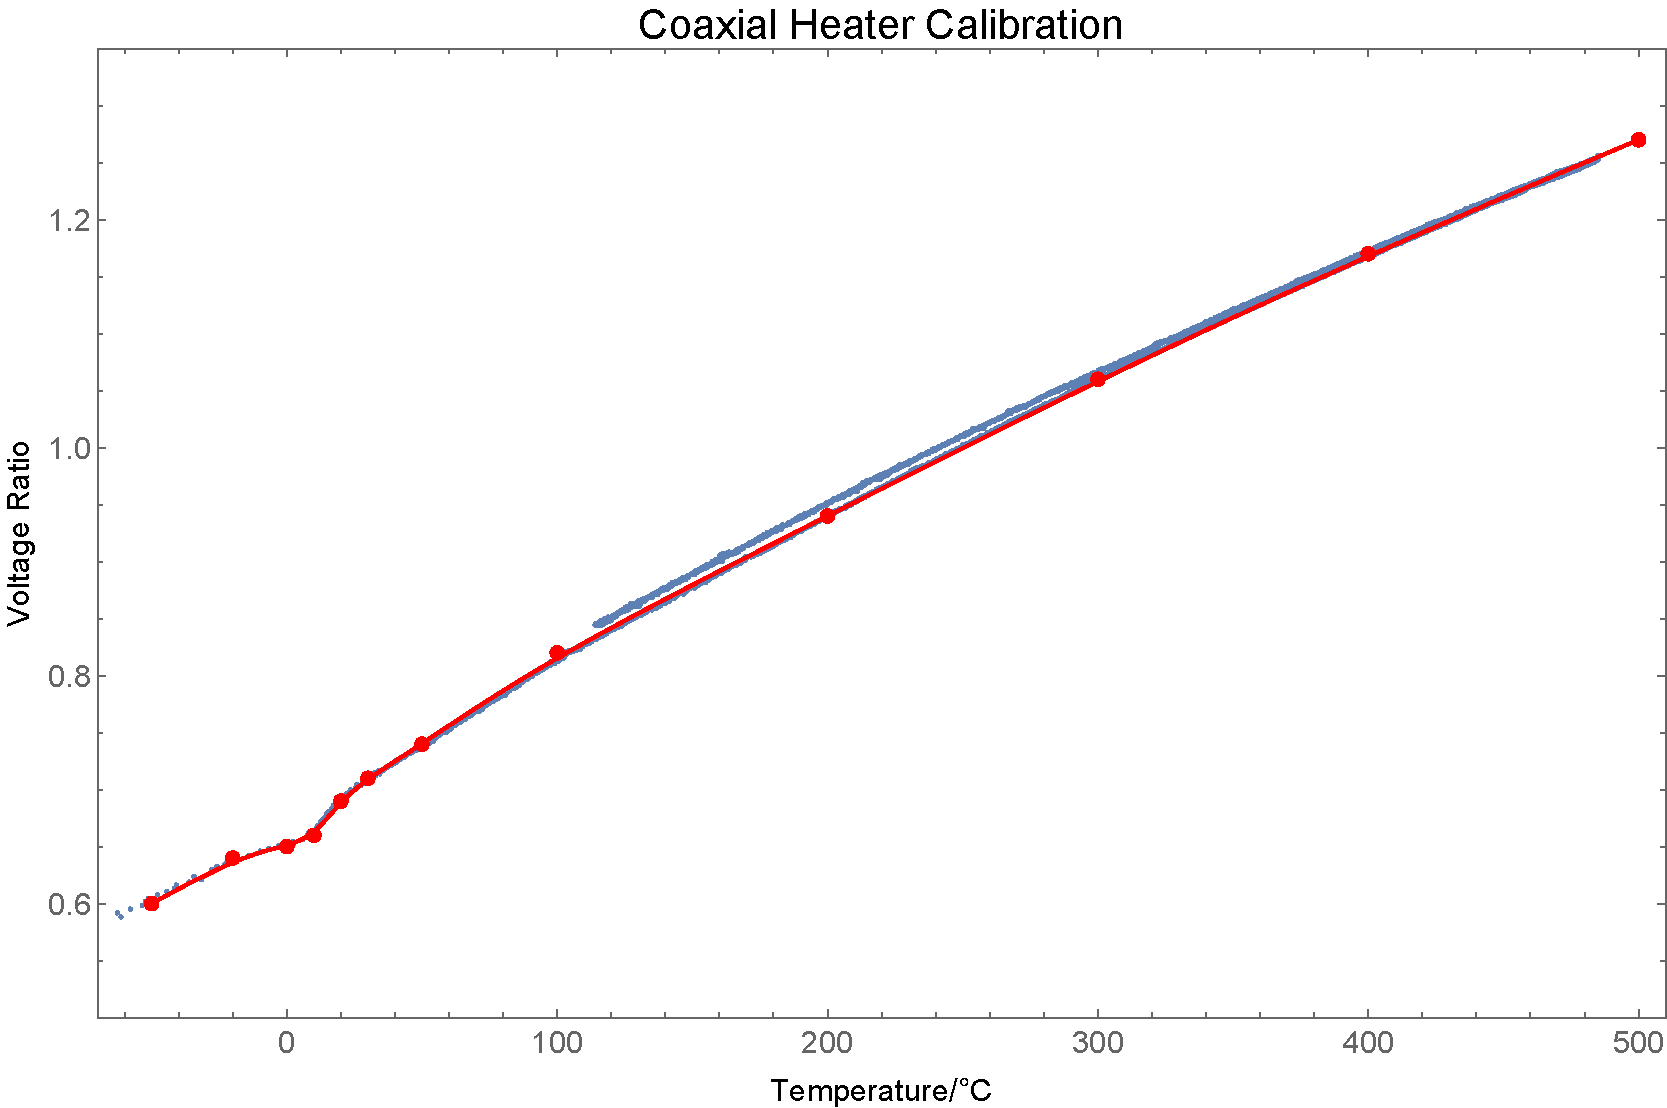
\includegraphics[width=0.8\textwidth]{Figures/2019_07_12_B-spline_fit_CPlot.pdf}
	\decoRule
	\caption[Calibration curve of the coaxial heater]{Calibration curve for the coaxial heater.}	
	\label{fig:CalibrationCurve}
\end{figure}

The second step of a calibration is to establish a \textbf{measurement result}
from an \textbf{indication}. It would be traditional to fit a mathematical
function such as a polynomial to the curve, but a numerical method was chosen
instead. We fitted a B-spline to the curve and extracted coordinates on the
curve from the B-spline (See Figure \ref{fig:MeasurementCurve}). An
interpolation function was then used to obtain the measurement result \(T\) from
the indication \(dV/V_b\).

\begin{figure}
	\centering
	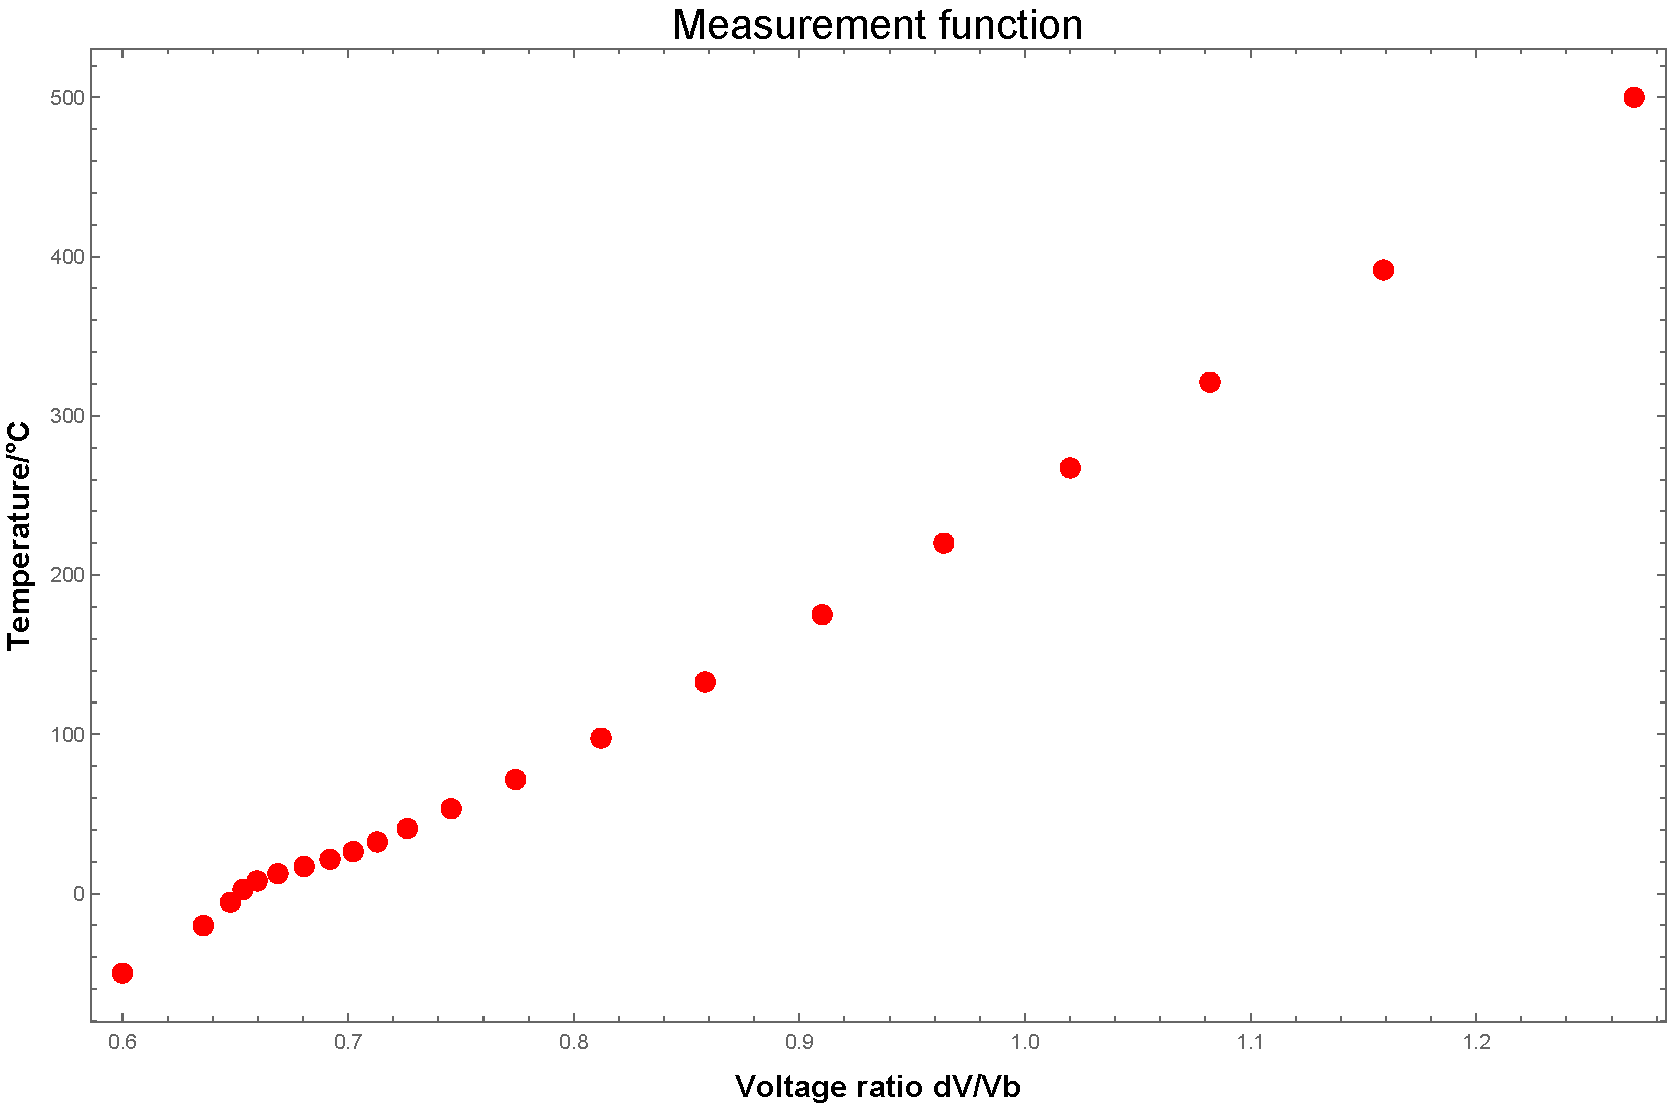
\includegraphics[width=0.8\textwidth]{Figures/2019_07_12_B-spline_fit_PPlot.pdf}
	\decoRule
	\caption[Measurement curve of the coaxial heater]{Measurement curve for the coaxial heater.}	
	\label{fig:MeasurementCurve}
\end{figure}

The calibration could be checked by setting the current through the coaxial
heater to a minimum, at which not enough heat is generated to affect its
temperature. Then the oven of the Varian 3300 GC could be set to a range of
different temperatures. Once equilibrium was reached the reported temperature of
the coaxial heater and the air bath temperature could be compared and the
calibration adjusted.

The technique of constructing a long, thin thermocouple probe allowed the
calibration of the coaxial heater, which makes it possible to translate
chromatographic methods. The probe has also proven useful in other applications,
for example proving overheating in a GC-MS transfer line.

\subsection{Cold spots}
\label{sec:ColdSpots}

For the fastest temperature programming with resistive heating, the heating
element should be as light as possible and carry the largest necessary current.
The current doing the heating must be carried to the coaxial heater using a feed
conductor. To prevent the feed conductor from heating up it must have a low
resistance, and this is achieved by making the conductor as 'thick' or as
'heavy' as necessary, meaning that it is constructed of a material with a high
mass per unit length.

Good electrical metallic conductors are invariably also good thermal conductors.
Therefore the area around the junction of the feed conductor to the coaxial
heater will always have a lower temperature than the nominal temperature of the
heater. In capillary GC this is undesirable: a cold spot in a column can wreak
havoc with retention times and peak shapes.

Conversely, if an attempt is made to reduce the contact area between the feed
conductor and the thin material of the coaxial heater, a hot spot might develop,
which could burn a hole in the coaxial heater tube or damage the column.

The electrical connection between the feed conductor and the coaxial heater was
therefore designed in the form of an externally heated block. This block was
kept at a higher temperature than the highest expected temperature of the
chromatographic temperature program. This prevented the formation of cold spots
in the coaxial heater, which might lead to cold spots in the column, while also
providing a large contact area so that hot spots do not develop. Each end of the
coaxial heater was fitted into one of two heated blocks, where it was brazed in
place. Each block had a brass tail, to which an electric feed-wire was
soft-soldered. Each block was heated by four \SI{100}{\watt}
Hotset\texttrademark{} electrical cartridge heaters, with dimensions of \SI{6.5
x 40}{\milli\metre}. The cartridge heaters were switched on and off by solid
state relays controlled from the computer. The temperature of the block was
monitored through a thermocouple mounted in a blind hole in the block and the
amount of power to the heaters was controlled by \keyword{pulse width
modulation} (PWM) implemented in software.
 
\subsection{Cold column}
\label{sec:ColdColumn}

In a cold GC stationary phase, the retention factor \(k'\) of a particular
compound can be very high. This means that the analytes migrate slowly relative
to the mobile phase. The lower the temperature, the higher \(k'\) becomes, so
that for very low temperatures the migration of the analyte becomes negligible.
In effect, the analytes are 'trapped'. This trapping, also called
\keyword{cryo-trapping} or \keyword{cryo-focusing} is useful in various aspects
of gas chromatography, such as two-stage thermal desorption or thermal
modulation in GC×GC.

%In one such
%application a programmable temperature vaporizing inlet (PTV) was used to trap
%complex hydrocarbon fractions from an SFC for injecting into a GC×GC system
%\autocite{Potgieter2013}.

In the SFC×GC instrument described here, cryo-trapping was used as the second
stage of a two-stage modulator. (The stop valve described in Section
\ref{sec:stopflow} represents the first stage.) The column was cooled down to
very low temperatures, which trapped any analytes eluting from the first
dimension in a narrow band on the GC column. Once the required amount of
fraction had been collected, the eluate flow from the first dimension was
stopped by closing the stop valve. Then the temperature ramp of the fast GC
would start. As the coaxial heater warmed up the column the values of \(k`\)
would decrease, and the narrow analyte band would start migrating.

The first SFC×GC chromatograph cooled the column by using the oven cryo-cooling
capability of the Varian 3300 GC \autocite{Venter2004, Venter2003}. The purpose
is to cool the GC column to sub-ambient temperatures, normally needed when
analysing volatile compounds. In such cases the \(k'\) values at or near room
temperature are too low to provide adequate retention, and the cryo-cooling
function permits temperature programs to start at sub-ambient temperatures.

The Varian 3300 cryo-cools its oven by injecting liquid carbon dioxide into the
oven's air circulation fan. The evaporating liquid carbon dioxide absorbs energy
from the air, which lowers the temperature of the air in the oven. A control
system controls the amount of carbon dioxide admitted and the amount of heat
added through the oven heaters, thereby keeping the oven at the required
temperature.

The cryo-cooling function can cool down the oven to cryo-trap analytes, but
there are two reasons why it is not suitable for practical trapping in SFC×GC.
The first reason is the quantity of coolant required: doing SFC×GC runs revealed
that about \SI{15}{\kilogram} of carbon dioxide was consumed per run. A standard
cylinder of carbon dioxide contains \SI{33}{\kilogram}, which implies that a new
cylinder would be required every two runs. Such a rate of use is much too high
for the intended application of the instrument. The second reason is that it is
much too slow. The time spent on cooling the oven and the column is time that
cannot be spent doing separations, and cooling a conventional GC oven takes a
lot of time: the Varian 3300's cryo-cooling function took \SI{30}{\second} to
cool the column down to a low starting temperature. A commercial
forced-convection system (``GC Chaser'' supplied by Zip Scientific) improves the
cool down time of an Agilent 6890 GC oven, taking 7 minutes instead of 16,
cooling down the oven from \SI{350}{\celsius} to \SI{30}{\celsius}.
Cooling the column in an air bath has the same drawbacks of low conductivity and
low heat capacity as air-bath heating has (see Section \ref{sec:RampRates}).

A system was therefore developed that injected liquid carbon dioxide into one
end of the space between the column and its coaxial heater, with the other end
open to the atmosphere. When the valve opens the space rapidly fills with liquid
carbon dioxide, while the pressure drops from \SI{55}{atm} in the cylinder to
\SI{1}{atm} at the outlet. The liquid boils, absorbing large quantities of heat
from the column and coaxial heater in the process, so that their temperatures
decrease rapidly. This system solves the speed and coolant consumption problems:
because the coolant is in direct contact with the parts that need to be cooled,
the cooling is rapid, and because the coolant is applied where it is needed,
only a small quantity is required.

The carbon dioxide for cooling the coaxial heater was introduced through the
same heated block that provided the electrical connection (see Section
\ref{sec:ColdSpots}). A T-piece design allowed the liquid carbon dioxide to be
admitted to the end of the coaxial heater, which was brazed to the block. A
micro-union brazed to the block sealed the column's exit port, and the liquid
carbon dioxide entered along the side of the T (Figure \ref{fig:ManifoldDims}
and Figure \ref{fig:ManifoldAssy}). A metering valve allowed the flow rate of
the coolant to be adjusted, and a computer-controlled solenoid valve switched
the flow on or off.

\subsubsection{Cryogen supply}

The carbon dioxide for cooling was supplied by Afrox in high-pressure
cylinders each containing 33kg of technical grade carbon dioxide. Each cylinder
was internally equipped with a \keyword{dip tube}, a tube that extends from the
valve at the top of the cylinder to the bottom of the cylinder. This ensures
that when the valve is opened, liquid carbon dioxide is delivered.

Experience taught that for repeatable cooling, the source of liquid carbon
dioxide had to be near the solenoid valve. If this was not the case, when the
valve was opened initially only carbon dioxide gas would be admitted, followed
by a mixture of gas and liquid, and only finally liquid. (This is similar to the
common experience of opening a water tap after a municipal water supply
interruption: a lot of gurgling and spitting before a reliable stream of water
flows from the tap.) Such unreliable coolant flow gives unreliable cooling.
To solve this problem we installed a reservoir for liquid carbon dioxide on top
of the GC. The problem of filling a receptacle with liquid carbon dioxide was
described in Section \ref{sec:CO2Pump}, so the final design of the reservoir
took the form of a coil of copper tube immersed in a circulating coolant (Figure
\ref{fig:CryogenReservoir}). Mounting the reservoir above the cut-off valve
allows the liquid to collect at the bottom and allow gas to collect at the top,
so that when the valve opens the flow into the coaxial heater contains only
liquid.

\subsection{Column mounting}

The T-piece blocks described in Section \ref{sec:ColdSpots} and Section
\ref{sec:ColdColumn} above and also depicted in Figure \ref{fig:ManifoldAssy}
acted as electrical connections for the coaxial heater and as injection point
for coolant. The block is heavy compared to the coaxial heater and column, and
also has to absorb the forces of the coolant inlet tube and the electrical
connections. The column runs from the heated inlet/detector to a heated T-piece
block, and in between it should not be exposed to any low-temperature cold
spots, therefore the gap between the T-piece block and the inlet/detector should
be quite small, but the gap cannot be zero, because electrical isolation needs
to be maintained. Also, fused-silica capillary columns are fragile and
misalignment causes them to break. Therefore, mechanically stiff and accurate
mounting was needed for the T-piece blocks to allow the precise but adjustable
alignment of the T-piece blocks with the inlet/detector.

The final design for mounting the T-piece blocks was a pair of parallel rails.
These rails were held in place in the Varian 3300 oven by friction, so that they
could be adjusted and removed as necessary, yet were stiff enough to transfer
the necessary forces without deflecting. The pointed ends of the rails pressed
against a solid aluminium plate used as the floor of the oven, and at the top
adjustable points pressed against pressure plates which pressed against the roof
of the oven. Figure \ref{fig:RailsDrawing} shows a technical drawing of the
rails as designed.

The T-piece blocks were the electrical connections for the resistive coaxial
heater, which meant they needed to be electrically isolated, but they were also
heated, which meant that the insulation had to be resistant to heat. A
commercially available material that met these requirements was found in the
form of \keyword{silicon mica}, a composite material of mica and a silicone
resin. This material has a continuous operating temperature of at least
\SI{500}{\celsius}, making it ideally suited to GC applications. The silicon
mica is also machinable and can easily be shaped to the required design. 

The T-piece blocks were mounted on a pair of cars riding on the round-bar rails.
Each car was designed as a sandwich of plates of stainless steel and silicon
mica around a pair of brass bushes. Once assembled, the cars offered a set of
studs on to which the user could fit and bolt down the T-piece blocks. The
positions of the cars were determined by a locking collar on one of the rails.
Figure \ref{fig:CarsDrawing1} shows technical drawings of the cars that explain
the design.


\subsection{Heating control}

The amount of electrical power supplied to the coaxial heater was controlled by
a bank of six PNP 2N2955 transistors, connected in parallel to distribute their
heat dissipation. The final control signal was a voltage set either by a
potentiometer from the front panel, or by the computer. An operational amplifier
adjusted the current through the coaxial heater circuit so that a portion of the
voltage applied to the coaxial heater was equal to the set-point voltage. By
varying the set-point voltage the current through the coaxial heater can be
controlled to provide any desired amount of heat (\(P = I^2R\)).

\subsubsection{Temperature monitoring}

Independent of the amount of power dissipated in the coaxial heater, the current
through the reference resistor was compared to the current through the column.
This ratio corresponds to the resistance of the coaxial heater. This resistance
is a function of the temperature of the heater. Through the calibration
procedure described in \ref{sec:Calibration} the temperature of the coaxial
heater can be calculated. The computer can do this fast enough to continuously
provide temperature as a process variable to the control system.

\subsubsection{PID tuning}

A proportional-integral-derivative (PID) controller was used to calculate the
amount of power necessary to keep the temperature of the coaxial heater as close
to the temperature set-point as possible. The temperature set-point, in turn,
was given by the desired chromatographic temperature ramp.

The process of determining the best calculation by the PID is called
\keyword{tuning}, and usually consists of determining the optimum values of a few
parameters. Tuning PID controllers is a complex sub-discipline of process
engineering, and outside the scope of this project, but for practical purposes
we used a privately published step-by-step tuning method \autocite{Peacock2008}
which is a version of the Cohen-Coon tuning method.

Figure \ref{fig:LoopTuning} shows the effect of an improved loop tuning. 

\begin{figure}
	\centering
	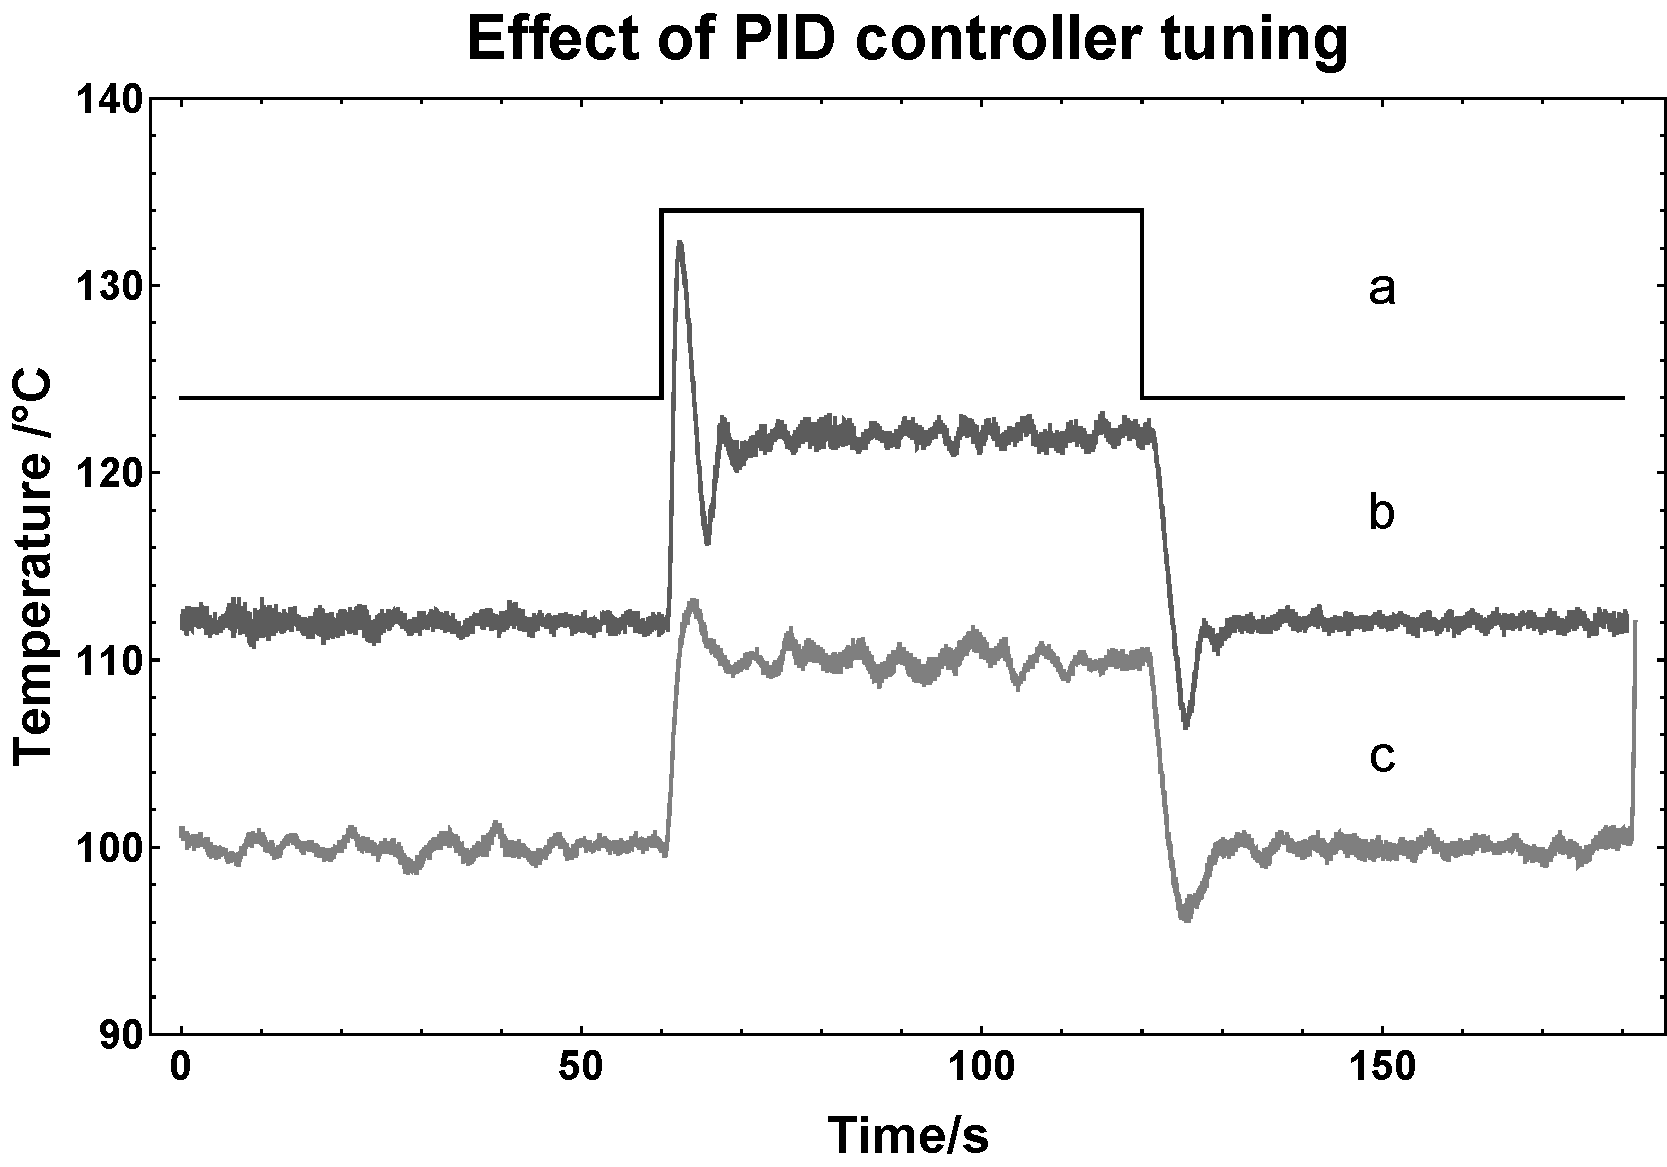
\includegraphics[width=0.8\textwidth]{Figures/LoopTuningGraph.pdf}
	\decoRule	
	\caption[Effect of controller tuning]{An illustration of effective PID
	controller tuning. The trace (a) represents the set point change over time and
	includes a step change. (b) Before tuning the temperature overshoots and then
	undershoots the step change in the set point. (c) After the controller has been
	tuned the overshoot in response to a step change in the set point is minimized. }
	\label{fig:LoopTuning} 
\end{figure}

A properly tuned heater helps to improve the repeatability of the chromatography
through reliable temperature programs and prevents damage to the column due to
overheating during set point overshoots.

\subsubsection{Heating rates}

As discussed in Section \ref{sec:RampRates}, for fast temperature-programmed gas
chromatography the ramp rate needs to be in the order of thousands of degrees
Celsius per minute.

\begin{figure}
	\centering
	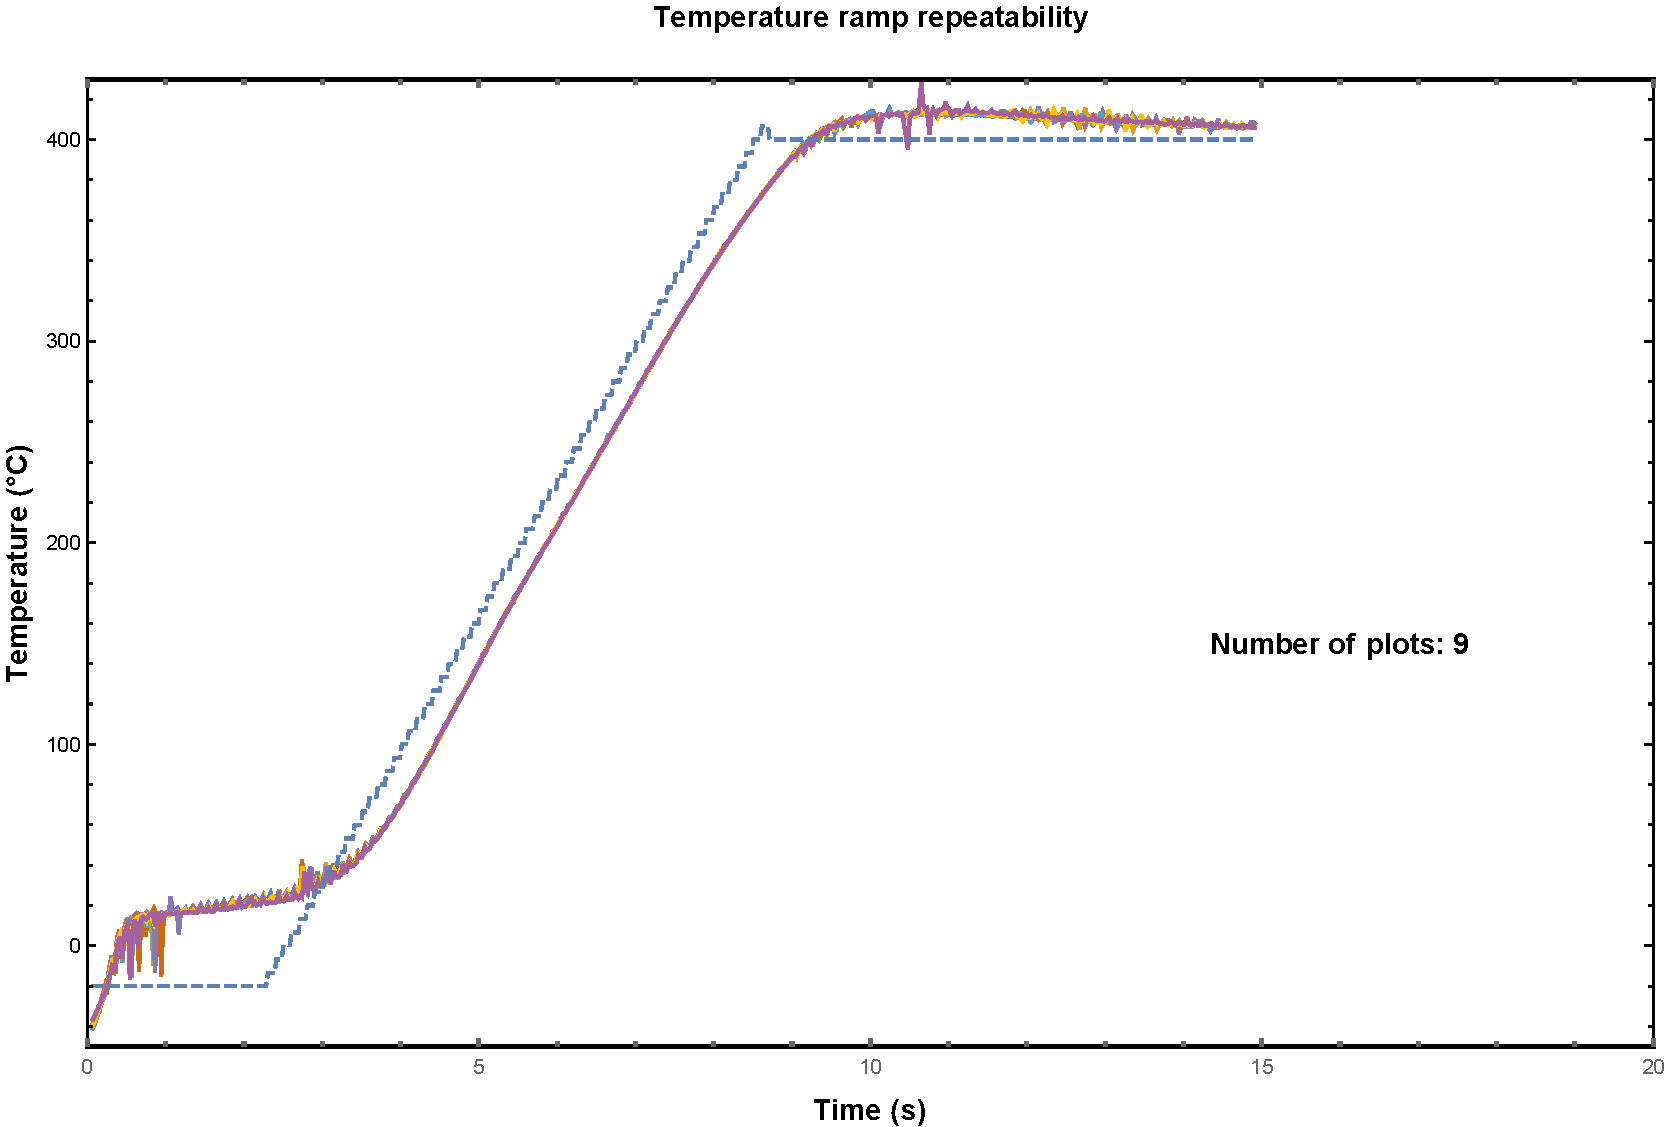
\includegraphics[width=0.8\textwidth]{Figures/high_rate_heating.pdf}
	\decoRule
		
\caption[Heating rate illustration]{A graph of 9 identical, consecutive
temperature ramps overlaid. The heating rate is \SI{4000}{\celsius\per\minute}.
The temperature follows (with some lag) the set point up to \SI{350}{\celsius}
before deviating noticeably.}

	\label{fig:4000K/min} 
\end{figure}

Figure \ref{fig:4000K/min} contains heating ramps executed by the coaxial
heater. The heating rate was \SI{4000}{\celsius\per\minute}, and there are no
significant differences between the 9 consecutive ramps.

\subsubsection{Cooling rates}

The project did not demand a precise knowledge of, or control over, the cooling
rate of the coaxial heater. The only requirement was that cooling should be as
fast as possible. The cooling rate could be adjusted through the metering valve,
and an optimum cooling rate of \SI{5100}{\celsius\per\minute} was achieved with
a carbon dioxide flow rate of around \SI{30}{\gram\per\minute}. This allowed the
column to be cooled down from \SI{350}{\celsius} to \SI{-20}{\celsius} in about
\SI{2}{\second}. At this rate the portion of the chromatographic cycle that is
not used for separation is dominated by fraction collection, and further cooling
rate increases will not significantly reduce sample throughput.

\todo{Find a place to put estimate of total coolant consumption for chromatogram.}

\section{Detector}

The detector used in this fast GC was an unmodified Varian\texttrademark{} 3300
flame ionization detector (FID). The detector bias voltage was supplied by the
original electronics, but a stand-alone high-speed electrometer (V.G. Micromass
Ltd, Model M406-H) captured the signal, which was then conditioned by a
bench-top amplifier (V.G. Micromass Ltd, Model M406) before it was sent to the
computer. This electrometer and amplifier were fast enough to detect and amplify
the signals generated by the fast GC.

\section{Data acquisition and control software}

The whole SFC×GC instrument was controlled from a single PC, running a single
program. The program was written in LabVIEW 7.1\texttrademark{} (National
Instruments). This software was designed to interact very easily with the
National Instruments PCI-6014 multifunction data acquisition board. LabVIEW is a
\keyword{visual programming language}, so called because programs are created by
manipulating icons and wires on a screen, instead of typing text. This visual
aspect of it makes it very easy to develop user interfaces as
\keyword{virtual instruments} and get quick results. Figure \ref{fig:SFCGCFastVI}
shows the interface of the program used to control the SFC×GC instrument.

\begin{figure}
	\centering
	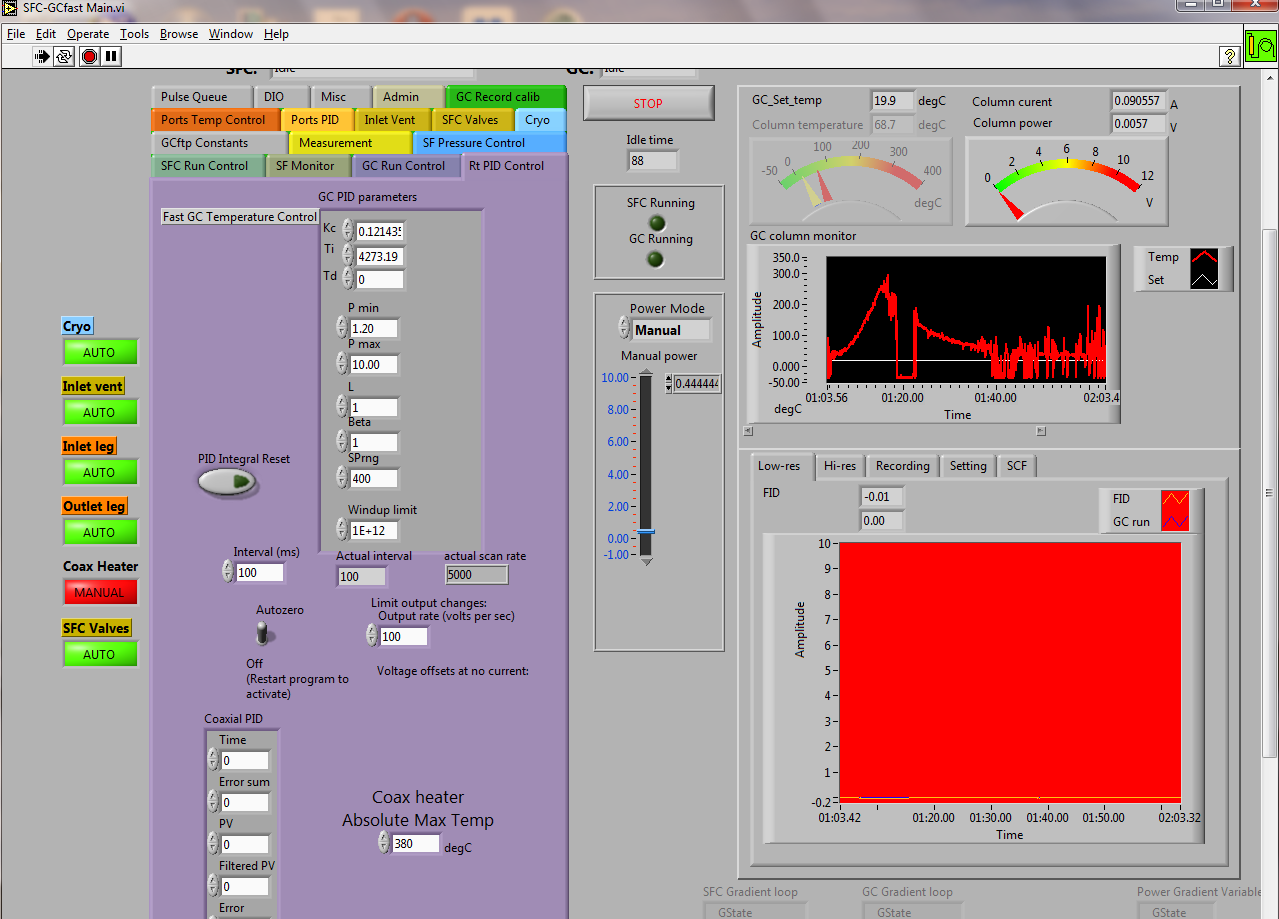
\includegraphics[width=0.8\textwidth]{Figures/Screenshot.png}
	\decoRule
	
	\caption[The main LabVIEW VI]{A screenshot of the LabVIEW virtual instrument
	used to control the SFC×GC instrument.}
	
	\label{fig:SFCGCFastVI}
\end{figure}


\section{Data structure}

In GC×GC, 2D data is recorded as a continuous FID output stream --- as if it is
a 1D GC chromatogram --- and later converted into a 2D chromatogram using
knowledge of the modulation period. For two reasons we could not use this
approach. Firstly, in our instrument the first (SFC) dimension runs in a
stop-flow mode making continuous data recording inappropriate. Secondly, the
duration of the cooling cycle varies, which would introduce unacceptable
variation in \textsuperscript{2}D retention times.

We therefore constructed 2D chromatograms by recording a GC run for each SFC
fraction injected. The \textsuperscript{1}D
retention times were recorded as the start times of each individual GC run.
The \textsuperscript{2}D retention times were measured from
the time the GC fast temperature program started. 

\section{Data visualization}
For data visualization we used the technical computing system Wolfram
Mathematica 11.3\texttrademark{}. Mathematica is an extremely powerful and broad
system, and we found it useful for its data manipulation and visualization
tools.

The collected data could be handled in different ways. One way was to split it
up into separate GC runs. Each individual GC run and its associated data could
then be examined using the \texttt{Manipulate[]} function (Figure
\ref{fig:SingleGC}).

\begin{figure}
	\centering
	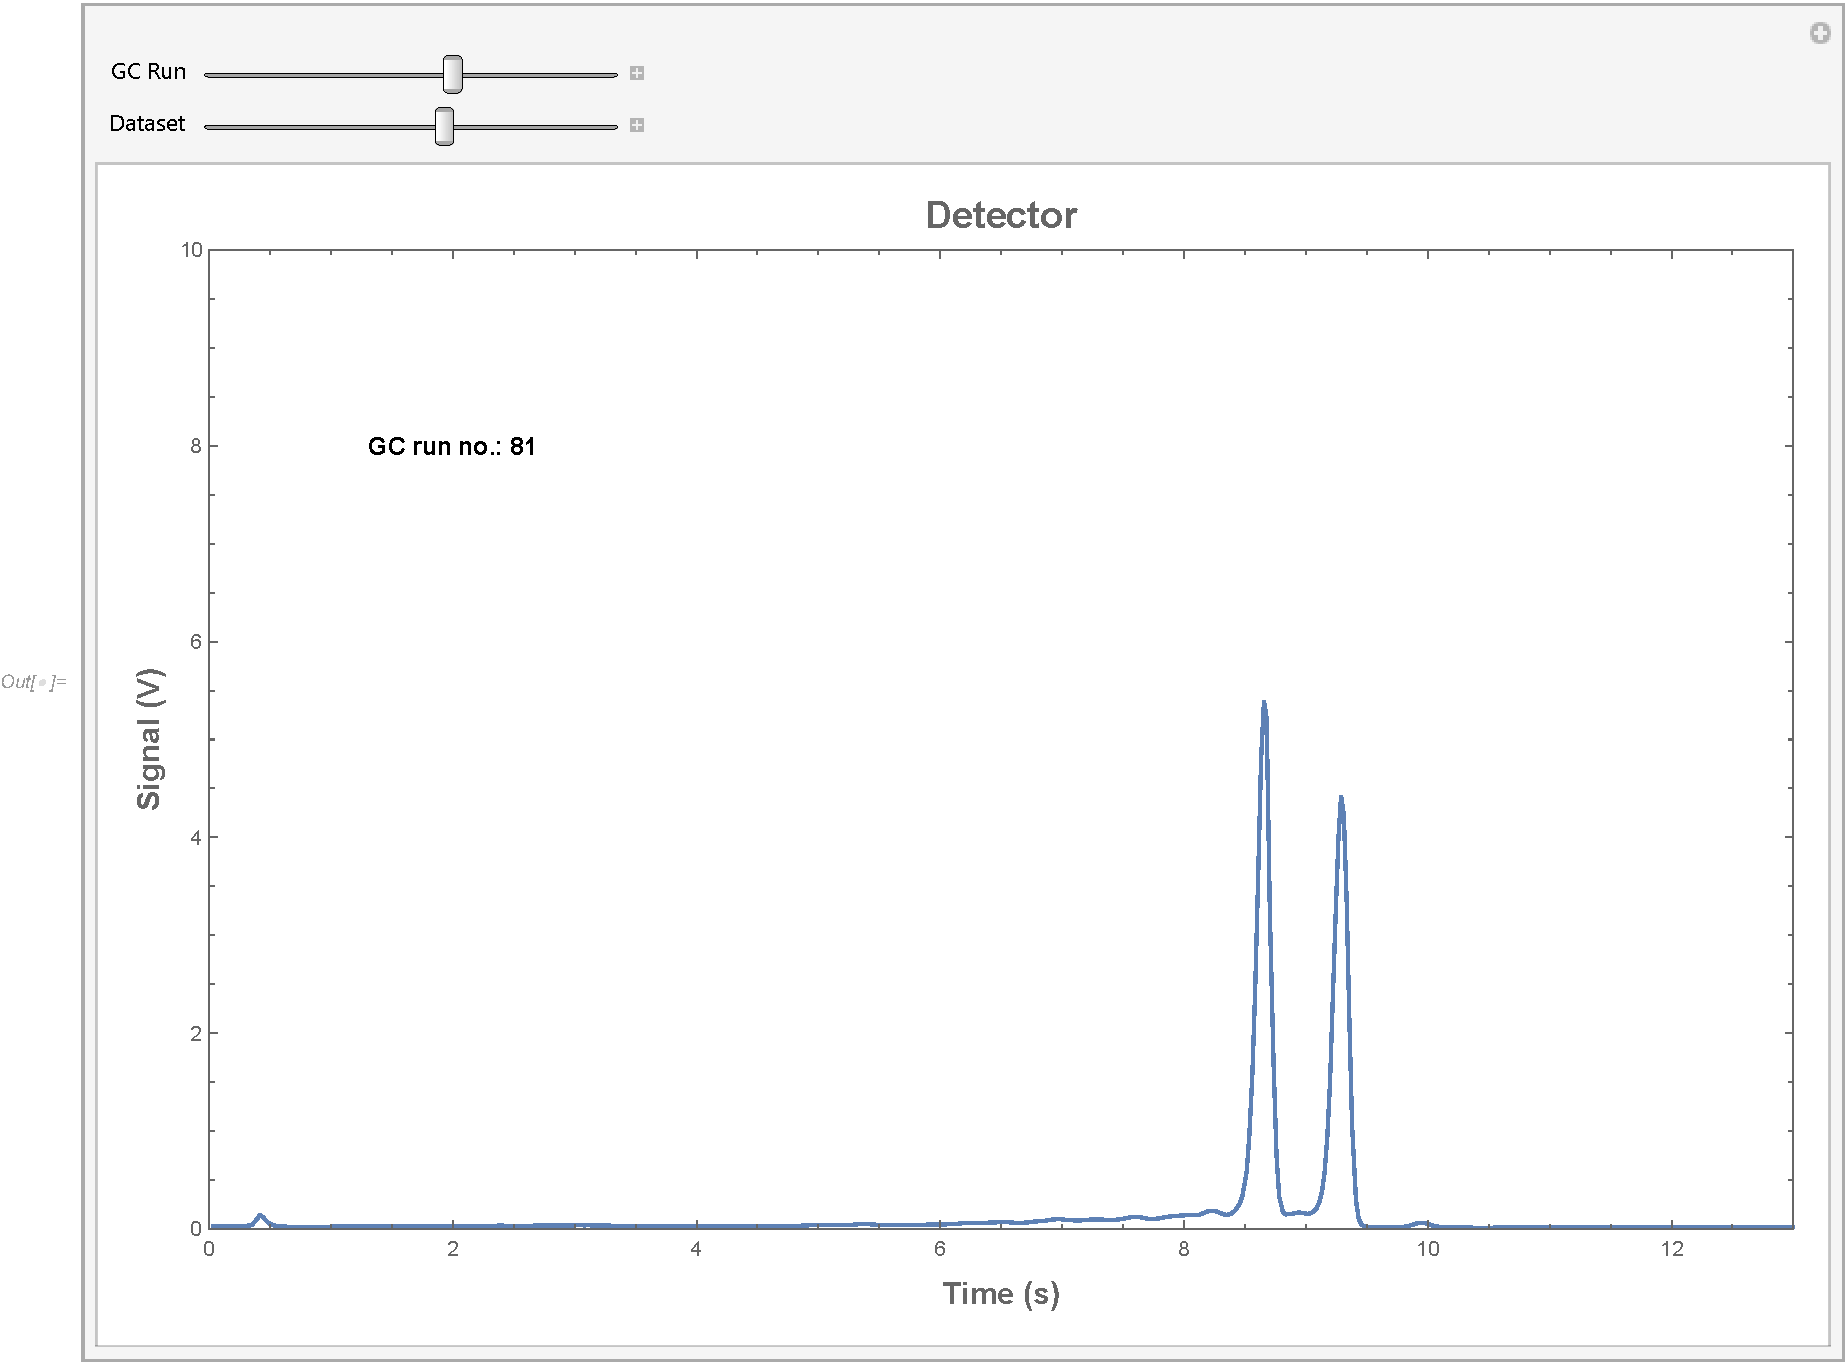
\includegraphics[width=0.8\textwidth]{Figures/Manipulate.pdf}
	\decoRule
	
	\caption[A single fast GC chromatogram ]{A single fast GC chromatogram, in a
	Mathematica \texttt{Manipulate[]} environment. The sliders can be used to select
	which GC run to view, and which data of that run. }
	
	\label{fig:SingleGC}
\end{figure}

Then the data could be re-arranged into a list of three-element lists, with
$^1$D retention time, $^2$D retention time, and detector signal as the elements
of the inner lists. The Mathematica functions \texttt{List3DPlot[]} and
\texttt{ContourPlot[]} could then be used to plot 3D chromatograms (Figure
\ref{fig:2DChromatogram}) or contour plots (Figure \ref{fig:Contourplot})
respectively.

\begin{figure}
	\centering
	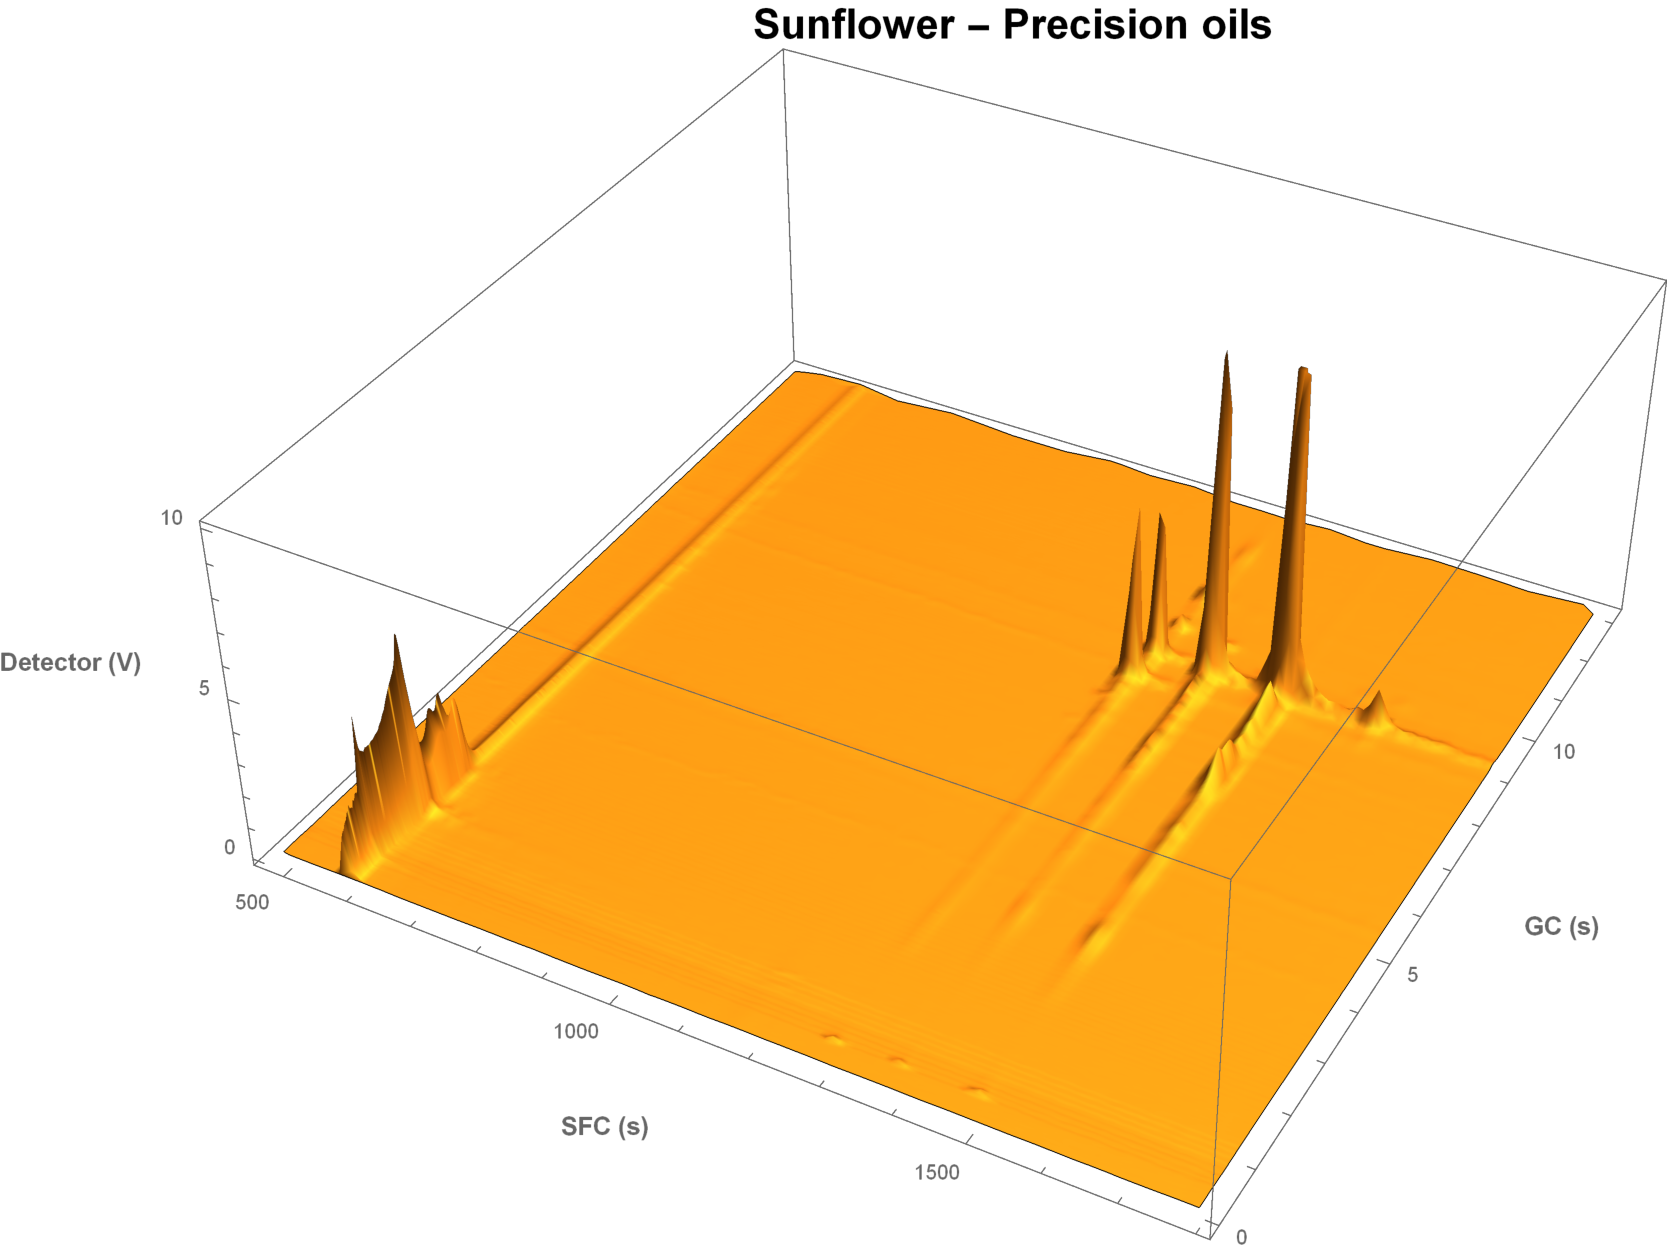
\includegraphics[width=0.8\textwidth]{Figures/2DChromatogram.pdf}
	\decoRule
	
\caption[A 2D SFC×GC chromatogram]{A 2D SFC×GC chromatogram of fatty acid methyl
esters of sunflower oil}
	
	\label{fig:2DChromatogram}
\end{figure}


\begin{figure}
	\centering
	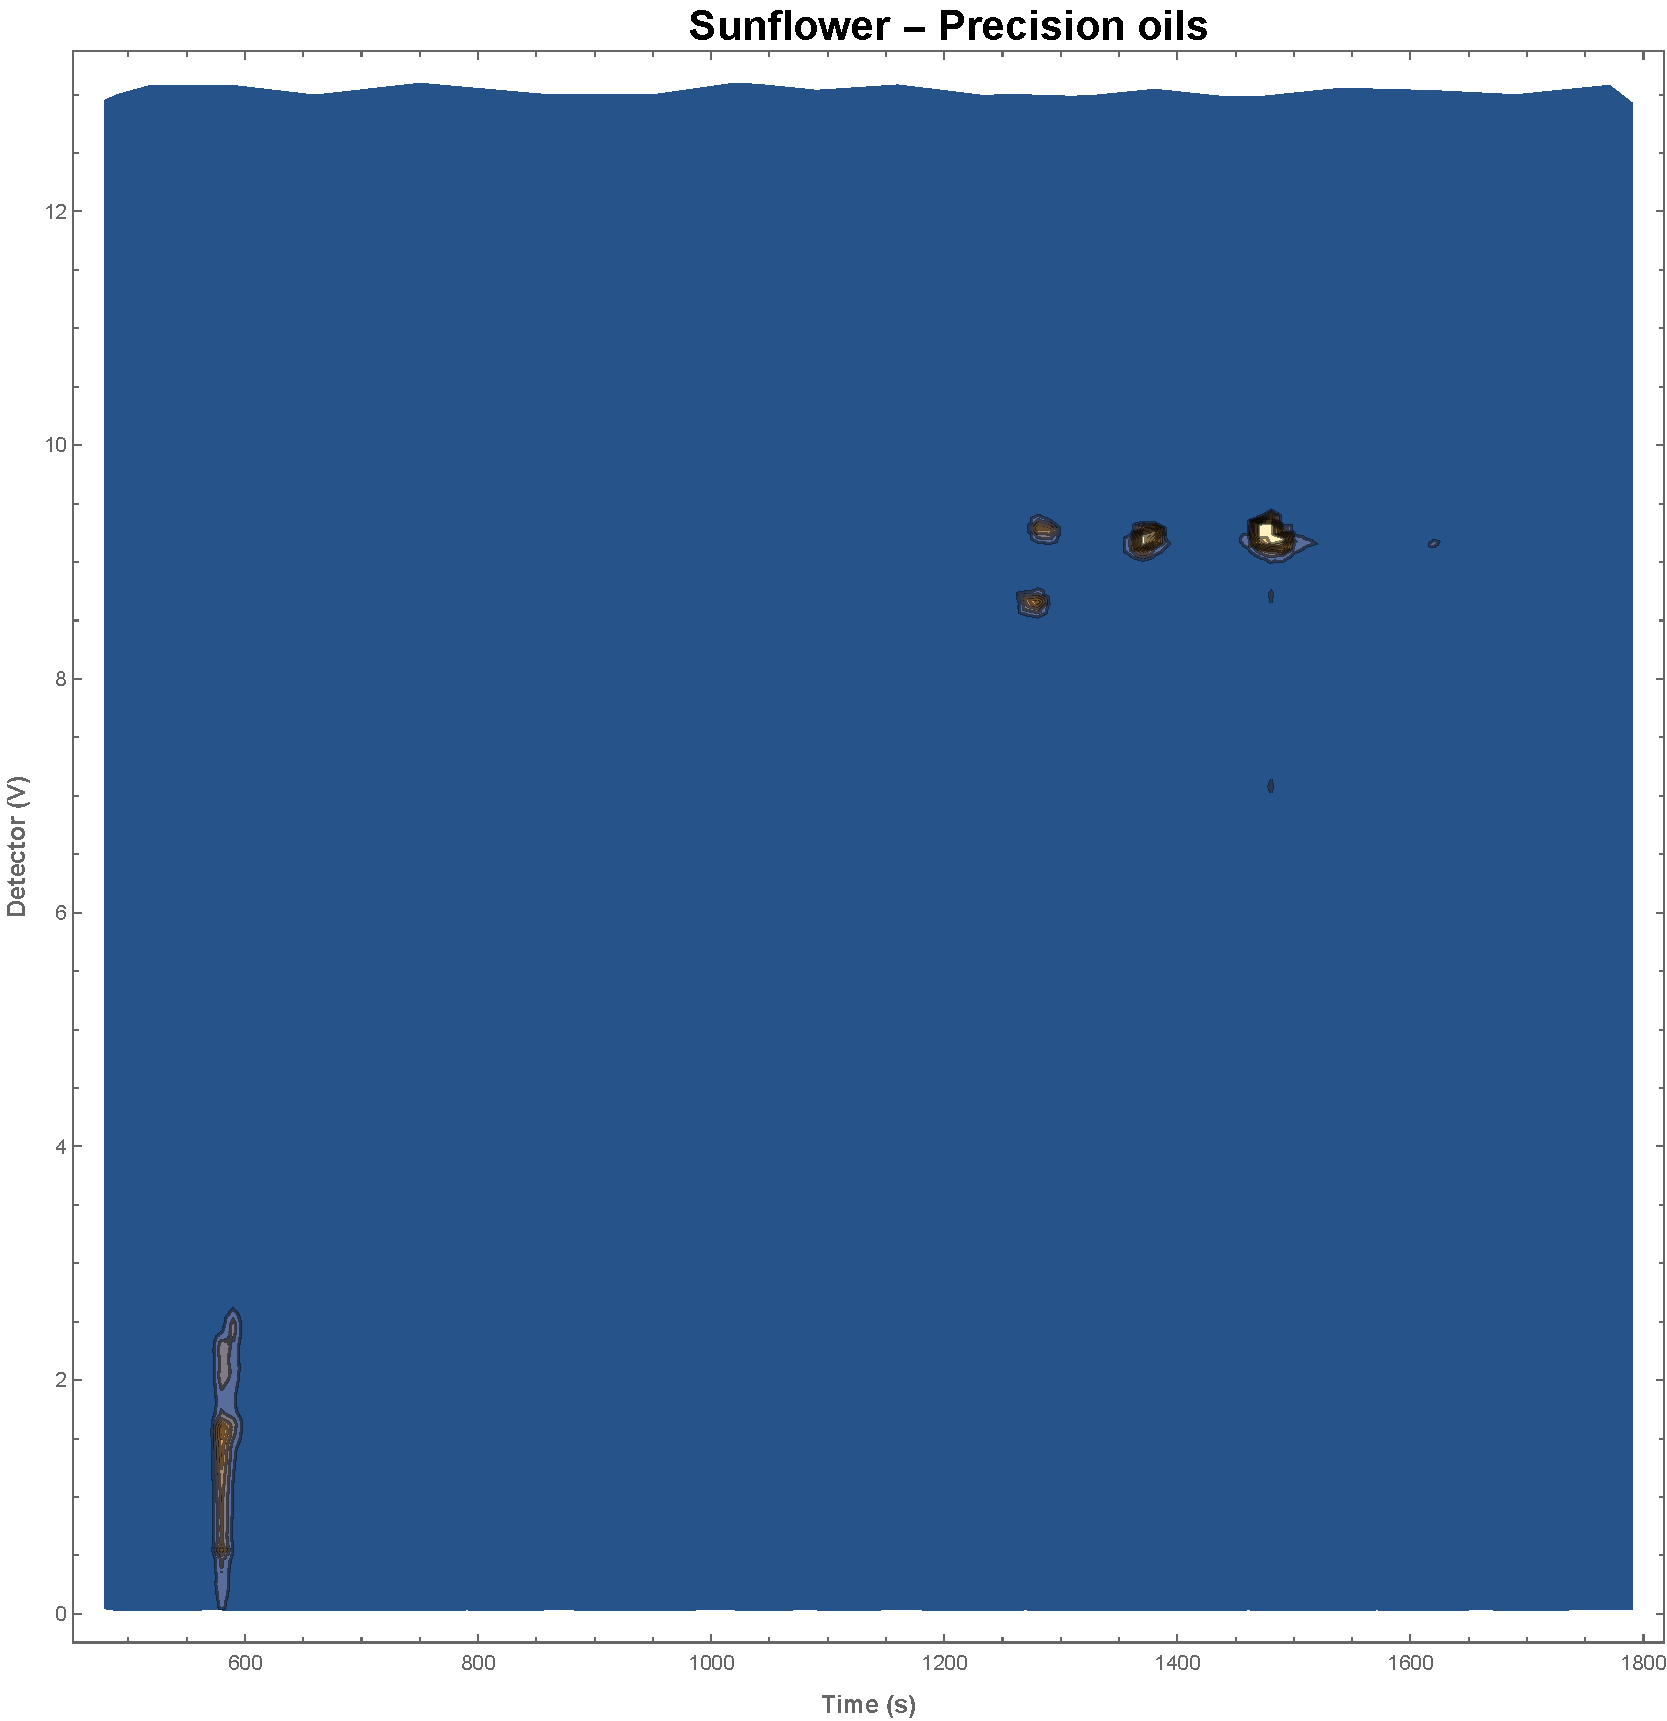
\includegraphics[width=\textwidth]{Figures/Contourplot.pdf}
	\decoRule
	
\caption[A 2D SFC×GC chromatogram]{The SFC×GC contour plot representation of the
2D chromatogram shown in Figure \ref{fig:2DChromatogram}.}
	
	\label{fig:Contourplot}
\end{figure}



